

\subsection{Valuation of markets under current market conditions}
This section presents the results using historical market data. Since two types of technologies and markets in three geographies were studied, there are a total of six distinct setups with each comprises serveral use-cases. In addition, we included a cost break-even analysis specifically for ESSs as few profitable opportunities were found due to high costs on battery stocks.

\subsubsection{ESS in Germany: opportunities hidden by adverse market design of balancing energy and frequency control}

\begin{figure}[h!]
	\centering
	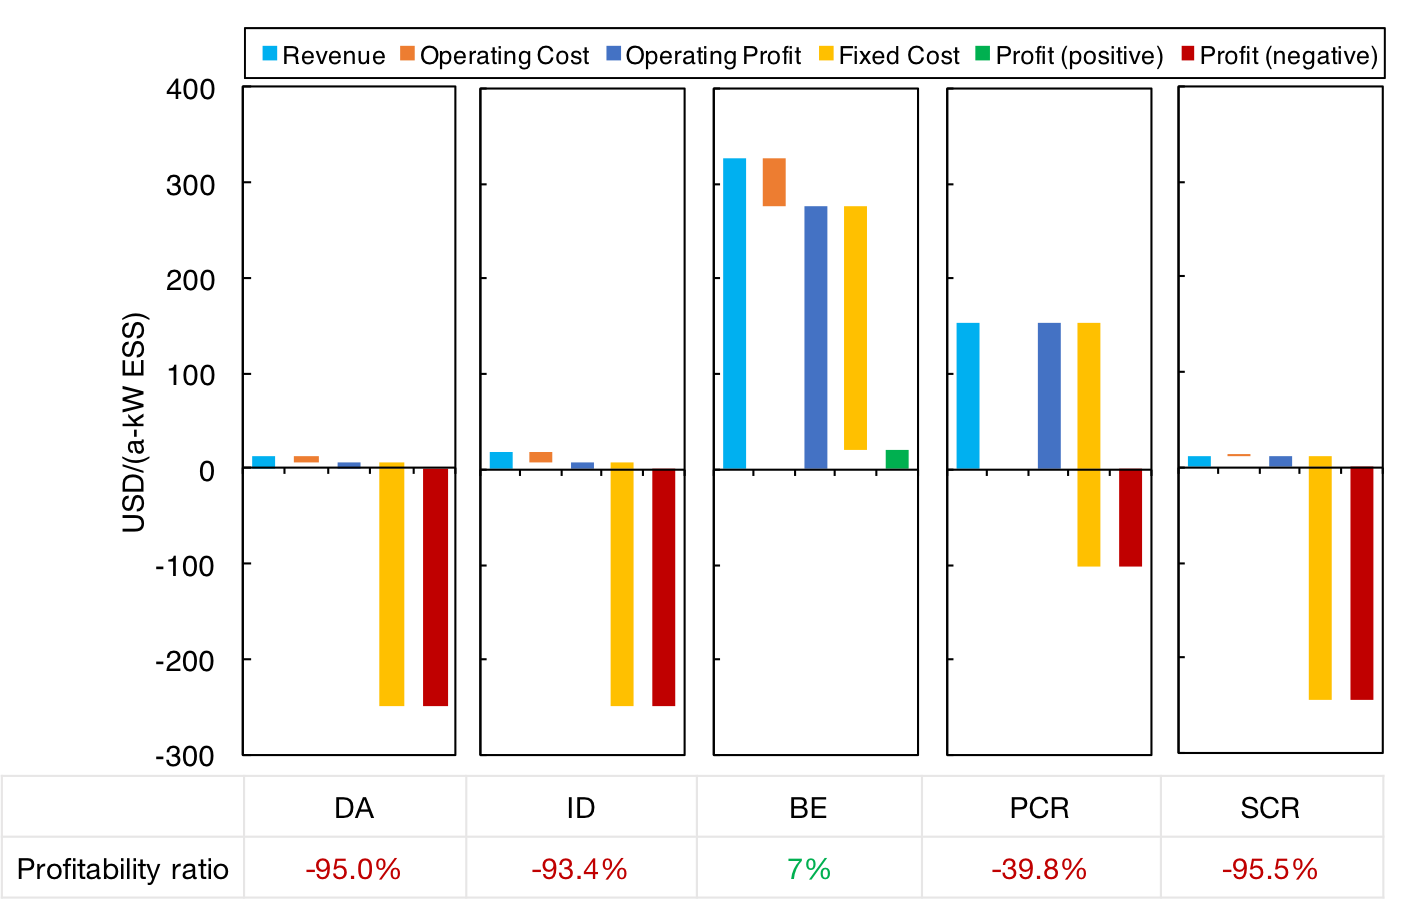
\includegraphics[width=0.9\linewidth]{Figures/Germany_ESS_profitability}
	\caption{Profitability of ESS in Germany electricity markets in the scenario of ``max. marginal Revenue"}
	\label{fig:germany-ess-profitability}
\end{figure}

\begin{figure}[h!]
	\centering
	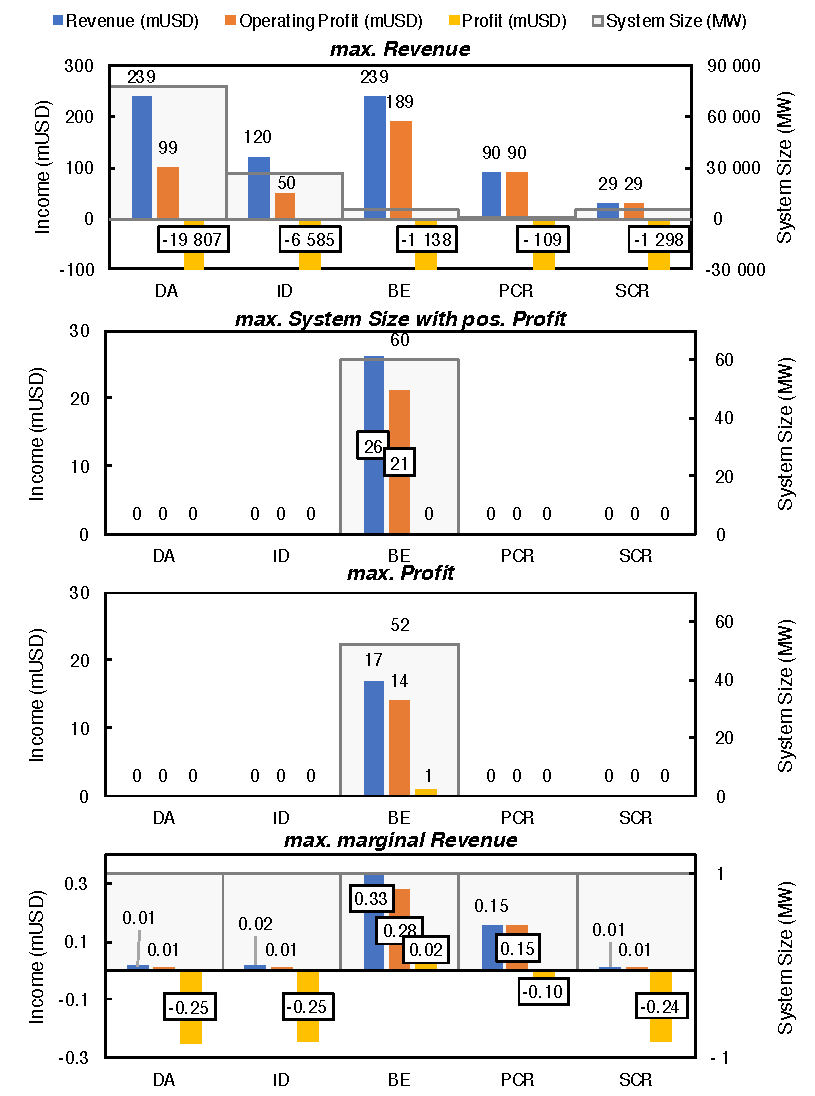
\includegraphics[width=0.9\linewidth]{Figures/Germany_ESS}
	\caption{Market size of ESS in Germany electricity markets in the scenario of ``max. Revenue"}
	\label{fig:germany-ess}
\end{figure}

As is discussed, profitability analysis can be performed using the scenario ``max. marginal Revenue", the results of which are depicted by Figure \ref{fig:germany-ess-profitability}. By showing values per unit ESS system installed, we can see the maximum unit return of ESS in Germany power markets. 

Meanwhile, with ample size of ESS, maximum potential market sizes can be derived, corresponding to the scenario ``max. Revenue".
Summarized by Figure \ref{fig:germany-ess}, annual cash flows are shown per MW consumption as normilzed values to the overal average consumption, \num{59138} MW . For example, the normalized revenue for arbitrage in day-ahead market is \num{4041} USD per year per MW consumption, which indicates the achievable revenue for a power system in Germay with 1 MW average load and corresponds to 239 mUSD/a in whole German market by mutiplying the base of \num{59138} MW.

It was found that the only profitable case is delivering balancing energy. As is analyzed in Section \ref{sec:qualitative-analysis}, this case corresponds to the situation of self-balancing where the players turn to the flexibility resource in avoidance of charges by TSOs for their imbalances. We further analyzed the maximum profitable system size and maximum profit of using the pre-defined BESSs; see Figure \ref{fig:germany-ess-profitable-size}.

\begin{figure}[h!]
	\centering
	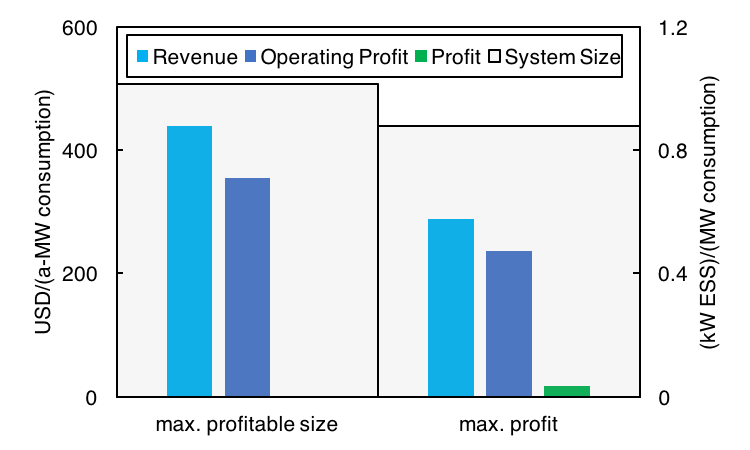
\includegraphics[width=0.9\linewidth]{Figures/Germany_ESS_profitable_size}
	\caption{Market size of ESS in Germany electricity markets in the scenario of ``max. System size with pos. Profit" and ``max. Profit"}
	\label{fig:germany-ess-profitable-size}
\end{figure}

It can be seen from Figure \ref{fig:germany-ess-profitable-size}, if being operated optimally BESSs with a size of up to 1 kW/(MW consumption) can generate profits by serving balancing energy, corresponding to a total 60MW in Germany. Nevertheless, it is challenging to be realized in practice. Market players do not have the right information to optimize their operational plans, since the balancing energy price, reBAP, is calculated \textit{ex-post} and highly volatile, hardly predictable, as is discussed in Section \ref{sec:qualitative-analysis}. On the contrary, if a system is designed to have ample size and tackle almost all imbalance events, it corresponds to a situation as the ``max. Revenue" scenario where we see negative profits from Figure \ref{fig:germany-ess-profitability}.

On the other hand, we noticed from Figure \ref{fig:germany-ess-profitability} that selling frequency control services to TSOs is less economically viable than using BESSs for self-balancing.The maximum marginal revenue from self-balance is significantly higher (33 times) than from selling frequency control products, while ideally the situation shall be reversed. The balancing energy charges are designed to recover the costs of activating frequency control services (calling for energy delivery) while the costs paid for securing capacity commitment are socialized, as have been fully discussed in Section \ref{sec:qualitative-analysis}. Theoretically, players shall get higher turnover in the frequency control markets than avoided balancing energy charges. Furthermore, the actual total payment for SCR in Germany is 176 mUSD in 2016 which is equavilent to \num{2976} USD/$(\text{a} \cdot \text{MW})$, while the maximum achievable revenue with BESSs are bounded at \num{490} USD/$(\text{a} \cdot \text{MW})$ as shown in Figure \ref{fig:germany-ess} with the rest 83.5\% of the market is intangible for BESSs . Our results imply that the current design of frequency control markets is neither economically efficient nor technically feasible to integrate the emerging BESS resources, which verifies our analysis in Section \ref{sec:qualitative-analysis}. We have argued that hurdles exist against emerging BESS to participate in frequency control markets with the non-energy-neutral signals and block-wise offering, especially for SCRs which demand significantly higher energy delivery than PCRs.

Facing either lack of information transparency in balancing energy charges or unfavorable market rules in frequency control markets, BESS players have no feasible options in the current market setup to make profits.

However, we may argue this situation shall not be long-lasting. We have already seen that certain amount of BESS will be a cheaper option to defer the expense on imbalance settlements compared to what are currently incurred. The market operators shall develop well-designed frameworks to encourage the participation of these resources that are beneficial to lower the overall system costs. In reality, there are indeed debates proposing possible solutions on this issue, e.g. letting TSOs who have the most abundance of information own and dispatch the storage resources\cite{He2012}, re-engineering the pricing mechanism of balancing energy\cite{Wartsila2014} and implementing favorable frequency control products for storage\cite{Megel2017}, etc.

As an implication for technology vendors, these possible movements on market designs shall be taken care of as it could suddenly turn over the feasibly profitability of using BESSs for balancing services.

Regarding arbitrages value in energy market, although the potential revenues are \num{4041} USD/$(\text{a} \cdot \text{MW})$ in day-ahead and \num{2029} USD/$(\text{a} \cdot \text{MW})$ in intra-day market, the losses would be incredibly high in order to materialize the revenue using BESSs; see Figure \ref{fig:germany-ess}. Even in the scenario of maximum unit return, the losses are about 10-20 times of the revenue; see Figure \ref{fig:germany-ess-profitability}. It is clear that the heavy investments on batteries cannot be recovered from making arbitrage in energy market. However, since the operating profits are always positive, if technology vendors can enable similar functions as BESS using technologies with smaller capital costs such as certain types of DR, it is still possible to make profits out of the market worth a total of over 300 mUSD per annum in Germany.

\begin{figure}[h!]
	\centering
	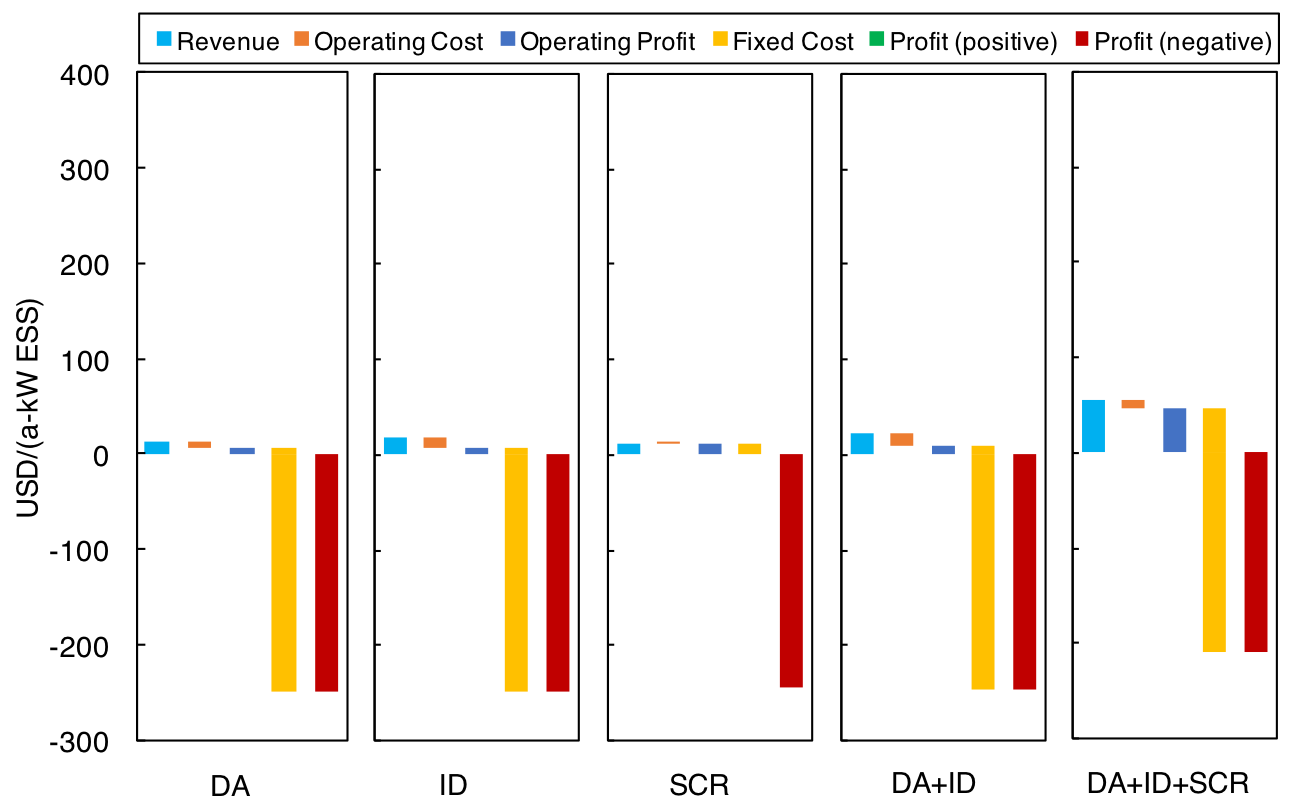
\includegraphics[width=0.95\linewidth]{Figures/Germany_ESS_profitability_multitasking}
	\caption{Profitability of ESS with multitasking in Germany electricity markets}
	\label{fig:germany-ess-multitasking-profitability}
\end{figure}

\begin{figure}[h!]
	\centering
	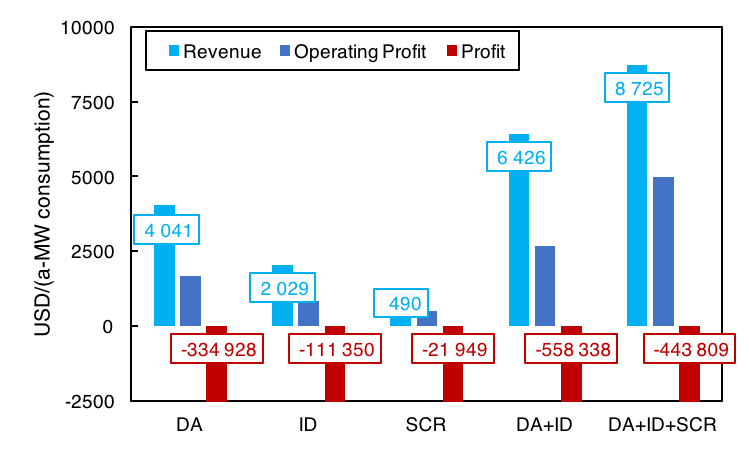
\includegraphics[width=0.95\linewidth]{Figures/Germany_ESS_multitasking}
	\caption{Market size of ESS with multitasking in Germany electricity markets}
	\label{fig:germany-ess-multitasking}
\end{figure}

As has been discussed qualitatively, in order to increase the profitability and find a way to neutralize the frequency control signals, we may stack operations in day-ahead, intra-day and secondary control reserve for multitasking. Figure \ref{fig:germany-ess-multitasking} shows the effects of multitasking.

While there are no significant synergies observed between day-ahead and intra-day markets (the unit returns remain unchanged in the scenario of maximum marginal revenue), stacking secondary control reserve with these two energy marketplaces will significantly improve the unit revenue (from 11 and 22 USD/$(\text{a} \cdot \text{MW})$ to 54 USD/$(\text{a} \cdot \text{MW})$) as well as the maximum revenue potential (from \num{6426} USD/$(\text{a} \cdot \text{MW})$ plus \num{490} USD/$(\text{a} \cdot \text{MW})$ to \num{8725} USD/$(\text{a} \cdot \text{MW})$). The maximum unit operating profit, as a consequence, raises by 4.5 times. The increment of maximum potential revenue of \num{2299} USD/$(\text{a} \cdot \text{MW})$ by stacking SCR on DA+ID indicates an additional revenue of \num{1809} USD/$(\text{a} \cdot \text{MW})$ are accessible for ESS in the SCR markets, reducing the intangible part from 83.5\% to 22.7\%. This corresponds to our previous analysis that the non-energy-neutral signal is indeed an issue for BESSs and has to be neutralized externally. Nonetheless, coping with third-party energy transactions requires the BESSs spare certain capacity to receive or release the energy, which reduces their availability in delivering SCR services. This is reflected on the result that this case with multitasking is still not profitable.

To sum up, while arbitrage is mainly constrained by costs on the technology side, making profits from balancing services is limited by adverse market frameworks although it has already shown its ability to make a positive contribution to the system. Technology vendors shall consider other technologies than BESSs or expect drastic cost reduction of BESSs to unlock the arbitrage value worth over a total of 300 mUSD/a in Germany. Profits from balancing market are more technically tangible, yet adjustments on market frameworks are required.

\subsubsection{ESS in PJM: successful practice of frequency control product design for flexibility}
The results of case studies in PJM power markets are illustrated in Figure \ref{fig:pjm-ess-profitability} and Figure \ref{fig:pjm-ess}.

\begin{figure}[h!]
	\centering
	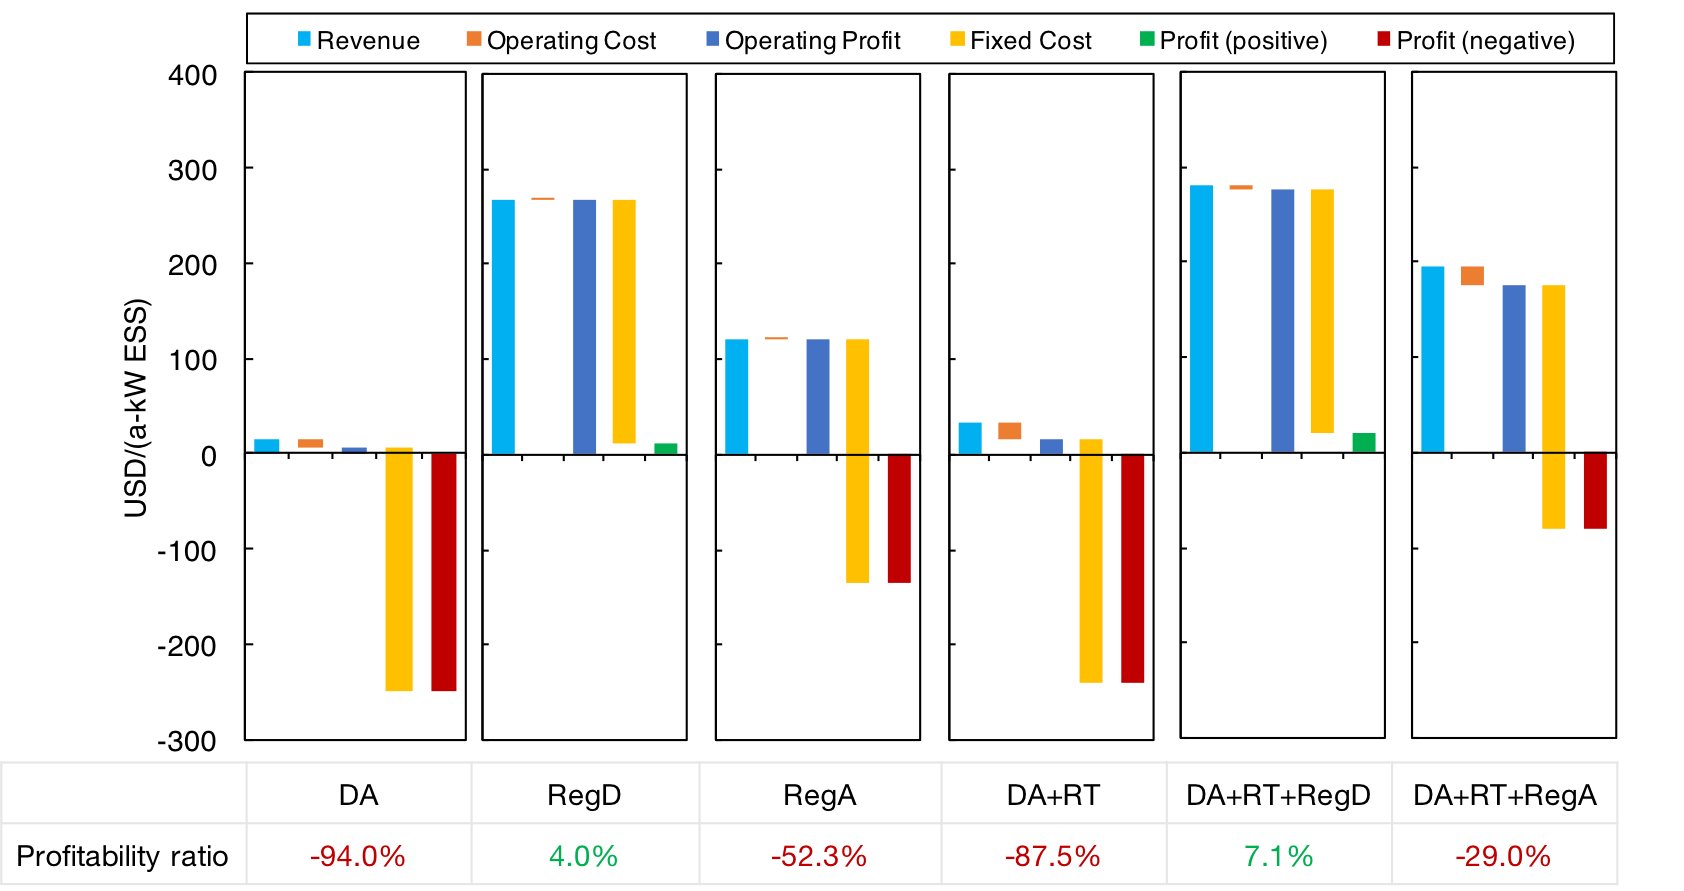
\includegraphics[width=0.9\linewidth]{Figures/PJM_ESS_profitability}
	\caption{Profitability of ESS in PJM electricity markets in the scenario of ``max. marginal Revenue"}
	\label{fig:pjm-ess-profitability}
\end{figure}

\begin{figure}[h!]
	\centering
	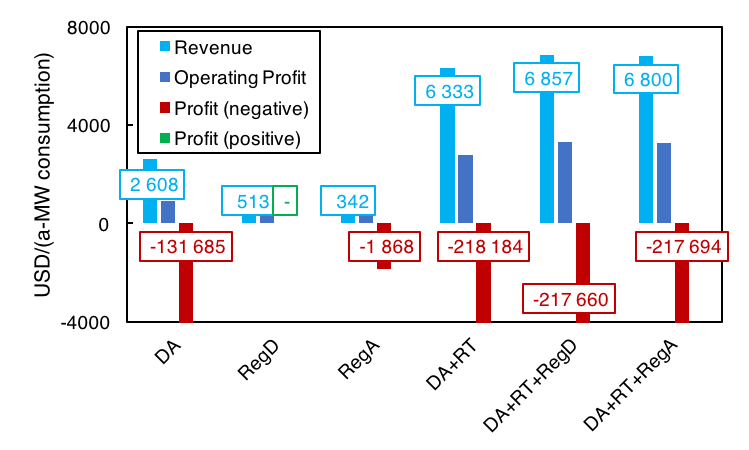
\includegraphics[width=0.9\linewidth]{Figures/PJM_ESS}
	\caption{Market size of ESS in PJM electricity markets in the scenario of ``max. Revenue"}
	\label{fig:pjm-ess}
\end{figure}

As we can clearly see, the RegD marketplace that is specially designed for emerging flexible technologies is indeed profitable. This shall give merit to PJM's RegD design including the conditional signal neutrality, operational flexibility, and higher price as a result of introducing mileage ratio and beneficial factor, as have sufficiently discussed in Section \ref{sec:qualitative-analysis}; also refer to Appendix \ref{sec:accounting-data-prepare}. The market with a total size of 513 USD/$(\text{a} \cdot \text{MW})$ can be wholly materialized by 2 kW/(MW consumption) BESSs without writing a loss, although the margin is very niche, barely above zero; see Figure \ref{fig:pjm-ess-profitable-size}.

\begin{figure}[h!]
	\centering
	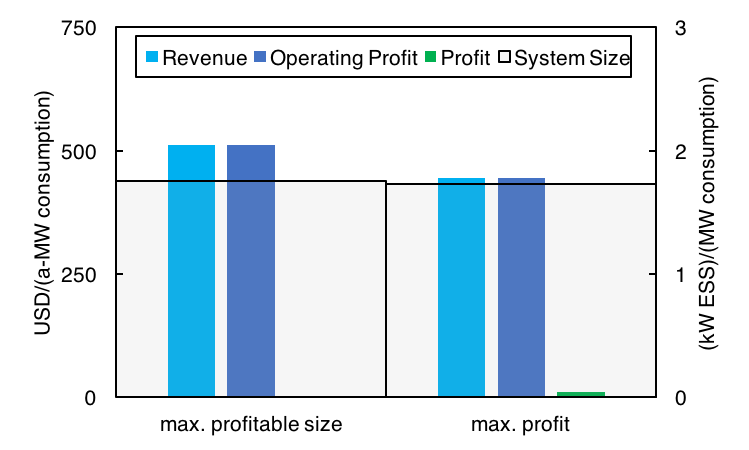
\includegraphics[width=0.9\linewidth]{Figures/PJM_ESS_profitable_size}
	\caption{Market size of ESS in PJM electricity markets in the scenario of ``max. System size with pos. Profit" and ``max. Profit"}
	\label{fig:pjm-ess-profitable-size}
\end{figure}

Those merits allow BESS players to offer RegD alone without coupled operations in the energy market which is currently necessary in Germany's power markets. As a result, stacking it with the energy market does not improve the profitability and tangible market size as significantly as in Germany. As we can see from an example shown by Figure \ref{fig:pjm-multitasking}, the system with pre-defined parameters in this study will have slightly surplus energy while strictly following the RegD signal. The SoC would raise quite slowly so that the resource can sustain the provision of RegD service over a long period (at least 84 hours shown in the chart) without involving transactions in energy markets. Trading in energy market is activated to leverage the arbitrage potential due to extreme price movements, which is however infrequent. Serving RegD is preferred for most of the time due its higher profitability. 

\begin{figure}[h!]
	\centering
	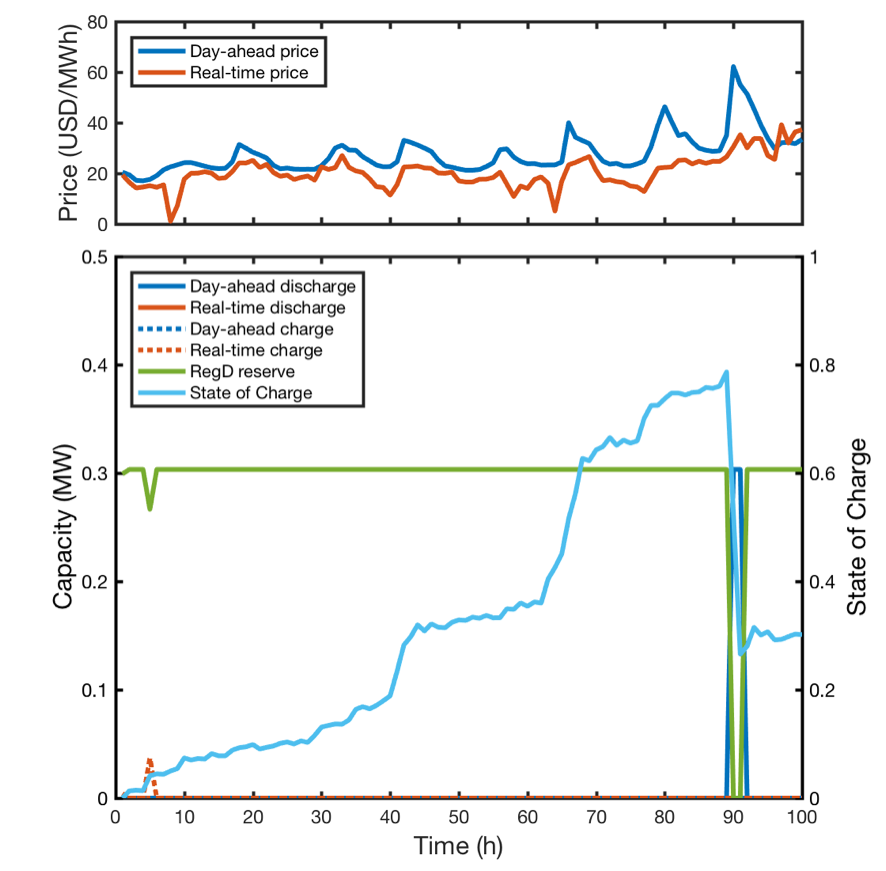
\includegraphics[width=0.9\linewidth]{Figures/PJM_multitasking_example}
	\caption{A example of operational plan with a 0.3MW battery energy storage system}
	\label{fig:pjm-multitasking}
\end{figure}

Apart from RegD market, there are no other profiting opportunities existing in PJM. Even the conventional regulation service RegA will create losses to BESS players.

Arbitrage in the energy market with flexibility through the so-called economic DR program, as is discussed in Section \ref{sec:qualitative-analysis}, is deemed not an ideal choice, especially in recent years when the electricity prices had fallen drastically with the shell gas revolution. As is discussed in Section \ref{sec:qualitative-analysis}, participating in the emergency DR program is a better option. However, the involvement of capacity market is not within our scope of quantifying the value, but the profiting mechanism is straightforward as is fully explained in the qualitative analysis. %It is also worthwhile to note that coupled operation in real-time and day-ahead markets will push the maximum revenue potential by 327 mUSD/a compared to 229 mUSD/a with participation in day-ahead market only.  

Overall, PJM shows a perfect example on how to offer incentives for the emerging storage technologies that are beneficial to the system, by implementing proper market frameworks such as the RegD and the  emergency DR program. For technology vendors, this market is already quite mature without spare space for new entrants unless significant changes may occur on market conditions, e.g. vast renewable penetration. Nonetheless, existing business cases in PJM may offer viable references for technology vendors to conduct similar practices in other markets. 
The upper-bounded values indicating the market potential are summarized in Table \ref{tab:pjm-summary}.


\subsubsection{ESS in NSW: most favorable market for arbitrage using flexibility yet still not profitable}

In New South Wales power markets, we only studied the real-time energy market, which was primarily due to the limitation of data availability.  Only information about total payment are available for the frequency control products. However, it was found that the overall size of these unaddressed markets are indeed negilible compared to the real-time energy market. The total payment in NSW's frequency control ancillary service (FCAS) market was worth 23.4 mUSD (2933 USD/$(\text{a} \cdot \text{MW})$) in 2016, which was equal to just 0.53\% of the total payment in the real-time energy market that was 4.4 bUSD (\num{551516} USD/$(\text{a} \cdot \text{MW})$). It was also much smaller than merely the arbitrage value, being 2.7\% of the revenue from arbitrage of \num{109301} USD/$(\text{a} \cdot \text{MW})$ as shown by Figure \ref{fig:nsw-ess}. This reflects the philosophy of market design to fully exploit the ability of real-time energy market to response to the system imbalances which are otherwise tackled by frequency control markets\cite{AEMO2010}\cite{McConnell2015}.
As a result, the price volatility in NSW's real-time energy market is significantly higher than the energy markets in other geographies, as is shown by Table \ref{tab:price-3-geo}.

\begin{table}[h!]
	\centering
	\begin{tabular}{l l R{3cm} R{4.5cm}}
		\hline
		\textbf{Geography} & \textbf{Market} & \textbf{Average price (USD/MWh)} & \textbf{Standard deviation of price (USD/MWh)} \\
		\hline
		NSW  & RT & 46.0 & 86.0 \\
		\hline
		\multirow{2}{*}{Germany} & DA & 34.8 & 15.0 \\
		\multirow{2}{*}{} & RT & 35.1 & 16.1 \\
		\hline
		\multirow{2}{*}{PJM} & DA & 30.0 & 11.6 \\
		\multirow{2}{*}{} & RT & 27.6 & 14.8 \\
		\hline
	\end{tabular}
\caption{The average and standard deviation of energy price in three geographies}\label{tab:price-3-geo}
\end{table}

\begin{figure}[h!]
	\centering
	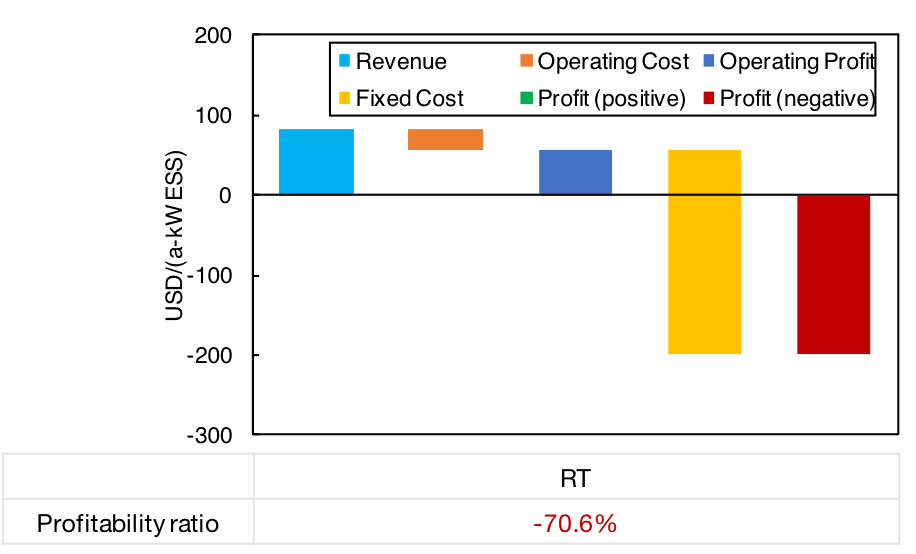
\includegraphics[width=0.9\linewidth]{Figures/NSW_ESS_profitability}
	\caption{Profitability of ESS in NSW electricity markets in the scenario of ``max. marginal Revenue"}
	\label{fig:nsw-ess-profitability}
\end{figure}

\begin{figure}[h!]
	\centering
	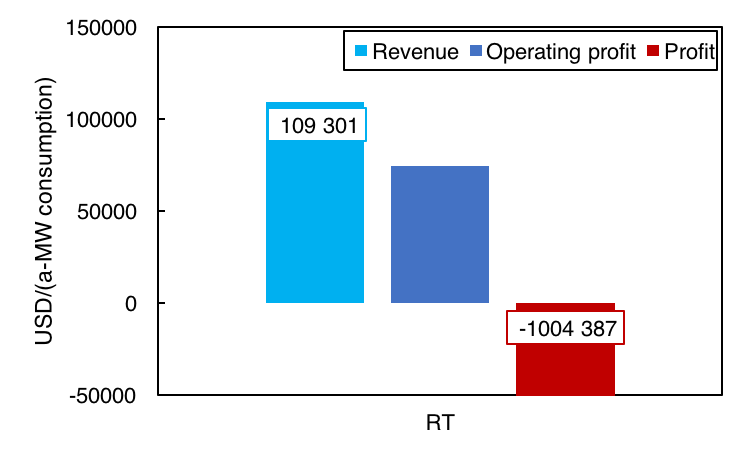
\includegraphics[width=0.9\linewidth]{Figures/NSW_ESS}
	\caption{Market size of ESS in NSW electricity markets in the scenario of ``max. Revenue"}
	\label{fig:nsw-ess}
\end{figure}

Such a volatile market is favorable for arbitrage. As we can see from Figure \ref{fig:nsw-ess-profitability} and \ref{fig:nsw-ess}.Profitability-wise the marginal revenue per unit system, 83 USD/$(\text{a} \cdot \text{kW ESS})$) is 2.4 times the value of arbitrage in DA+RT in PJM and 3.8 times the value of arbitrage in DA+ID in Germany. In terms of market potential, the maximum arbitrage revenue \num{109301} USD/$(\text{a} \cdot \text{MW})$) is roughly 17 times higher compared to either of those two arbitrage cases in Germany and PJM.

Nonetheless, even though in such a voltaile real-time energy market, it is still not a profitable business to deploy BESS in NSW for arbitrage.

\subsubsection{Cost reduction: where is the break-even point for arbitrage using BESSs}
According to the results above, using BESSs for balancing is already technically feasible while limitations lie on the aspect of market design. The value of arbitrage, however, is far away from being profitable due to high expenses on batteries. Overturn of arbitrage profitability using BESSs has to rely on reducing costs and changing market conditions. While the latter will be discussed in the proceeding section, hereby we present the results with reduced costs of battery stocks. 

In each geography, the case with the highest arbitrage potential was selected, which is respectively arbitrage in coupled day-ahead and intra-day market in Germany (DA+ID), arbitrage in coupled day-ahead and real-time market in PJM (DA+RT), arbitrage in real-time market in NSW (RT). We would show the maximum profitability ratio that is realized by a small size of BESS. Meanwhile  we would present the profitable revenue that is obtained as in the scenario of ``max. System Size with pos. Profit" to the maximum potential revenue derived from the scenario ``max. Revenue". It shall be pointed out the maximum revenue that is independent from costs would remain constant so adopted as the cardinal term to illustrate the growth of profitability. 

\begin{figure}[h!]
	\centering
	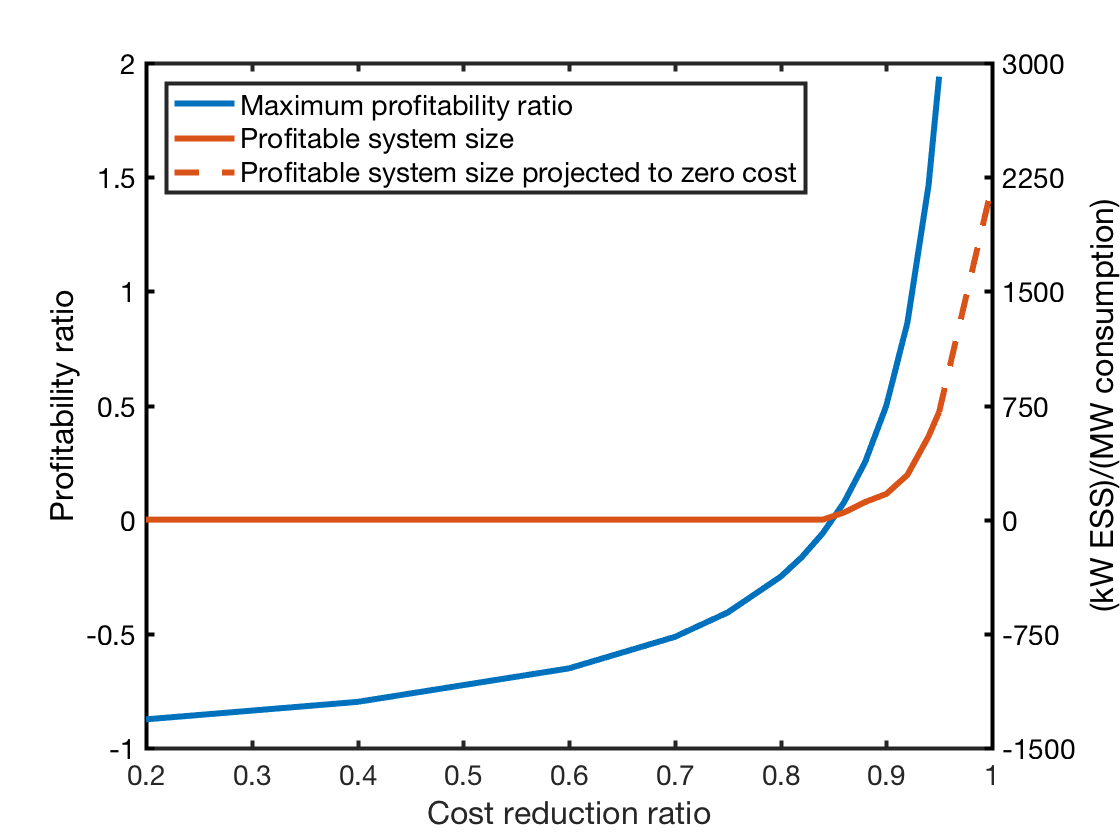
\includegraphics[width=0.9\linewidth]{Figures/CostReduction_Germany_ESS}
	\caption{Development of market size and profitability of arbitrage in coupled day-ahead and intra-day markets with reduced costs in Germany}
	\label{fig:germany-ess-costreduction}
\end{figure}

\begin{figure}[h!]
	\centering
	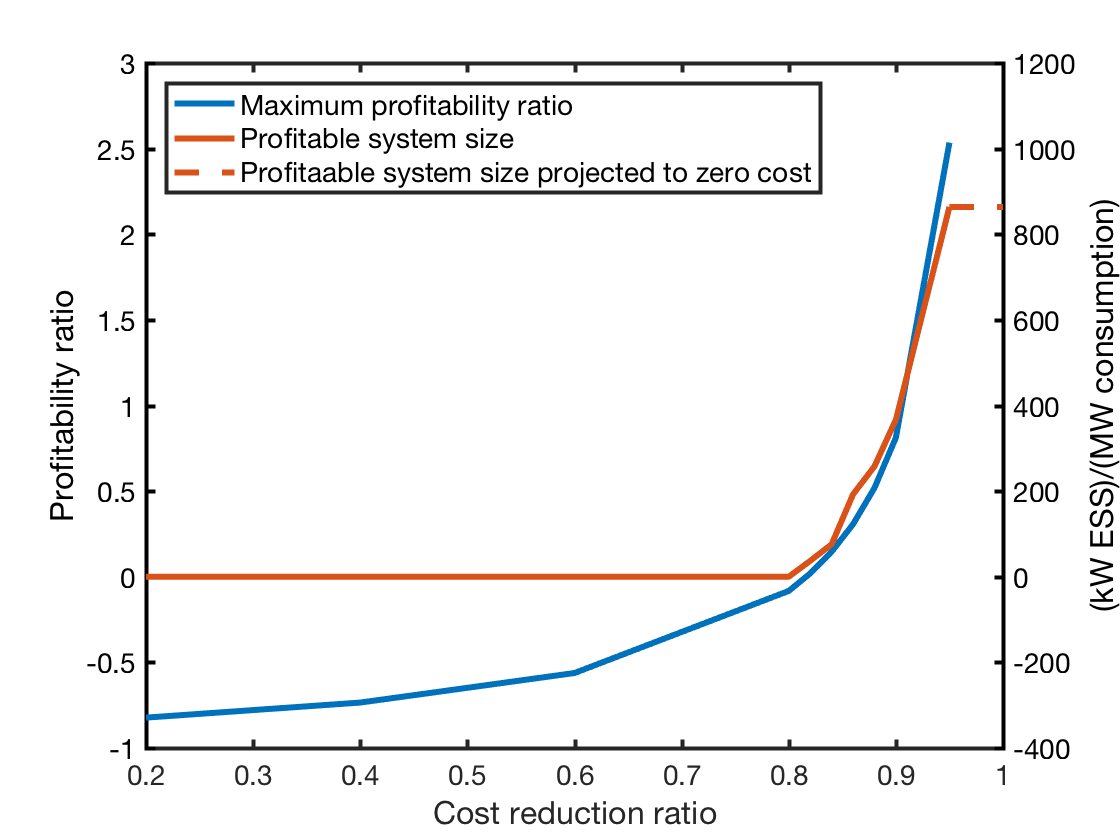
\includegraphics[width=0.9\linewidth]{Figures/CostReduction_PJM_ESS}
	\caption{Development of market size and profitability of arbitrage in coupled day-ahead and real-time markets with reduced costs in PJM}
	\label{fig:pjm-ess-costreduction}
\end{figure}

\begin{figure}[h!]
	\centering
	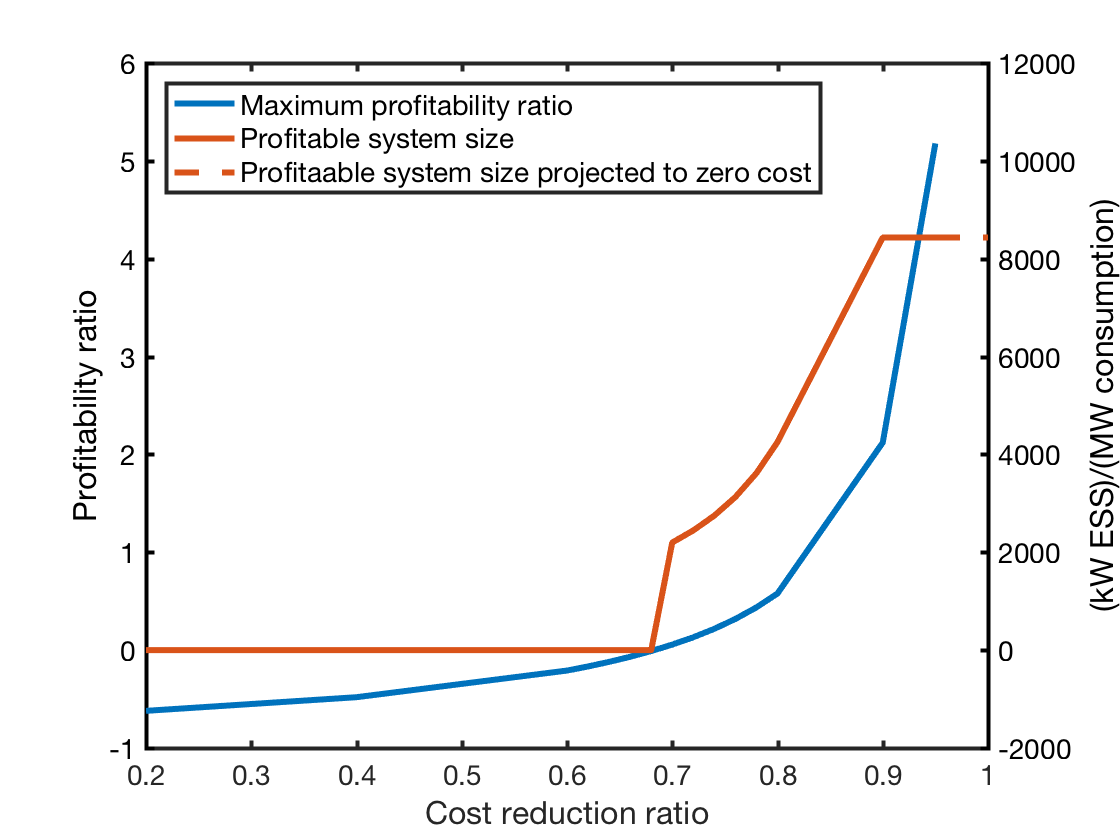
\includegraphics[width=0.9\linewidth]{Figures/CostReduction_NSW_ESS}
	\caption{Development of market size and profitability of arbitrage in real-time markets with reduced costs in NSW}
	\label{fig:nsw-ess-costreduction}
\end{figure}

Figure \ref{fig:germany-ess-costreduction} - \ref{fig:nsw-ess-costreduction} illustrate how the profitability and market size will evolve with cost reduced by up to 95\% in three geographies. The break-even point of costs is found to be 84\%, 81\% and 68\%, respectively in Germany, PJM and NSW. If we adopt the forecast made by IRENA\cite{IRENA2017} who predict the cost reduction by up to 60\% by 2030, none of these markets will be profitable for arbitrage by 2030. Even if we applied a constant learning rate of 14\% per annum according to \cite{Nykvist2015}, the break-even point will be realized in 12, 11 and 8 years, respectively in Germany, PJM and NSW. 

Moreover, it shall be noticed while the break-even point is just reached, the total profitable revenue will be almost at zero. To materialize the whole potential of arbitrage revenue, it requires a cost reduction of 95\%+, 95\% and 90\%, respectively in Germany, PJM and NSW, which is almost impossible to be realized in the foreseeable future.

As a conclusion, the cost reduction of BESS by learning effect alone will not turn over the profitability of arbitrage using BESSs in the near future. Unless revolutionary technical innovations happen, opportunities of arbitrage using BESS may only arise with drivers from the market, e.g. renewable penetrations, which are to be shown in Section \ref{sec:impact-market-condition}.

\subsubsection{EV2G in Germany: changeling in developing business model}
Implementing EV as a grid resource is not as straightforward as using generic ESSs that is discussed above. The main issue is that the energy demand for EV driving itself poses challenges to grid. It is not possible to deliver any services without incorporate a large-volume energy market. Therefore, the day-ahead energy market is always included for all the cases for EV2G. Moreover, in our case studies, it is found even with the day-ahead market, charging the EVs is not feasible while their number reached a certain level. In the optimization framework, the technology constraints would violate market constraints, especially the one that we set to restrict the activation of peak generation during non-peak hours, while the EV fleet grows beyond a certain scale. This corresponds to the situation where spare generation resources in the power system are not sufficient  to fulfill the energy needs of EVs. The electricity price may raise significantly in those scenarios compared to nowadays's level. As is shown by Figure \ref{fig:EV_nan_percentageg}, when the number of EV is higher than 1 million, it start to stress the electricity supply if the generation capacity remains at present level. 
\begin{figure}[h!]
	\centering
	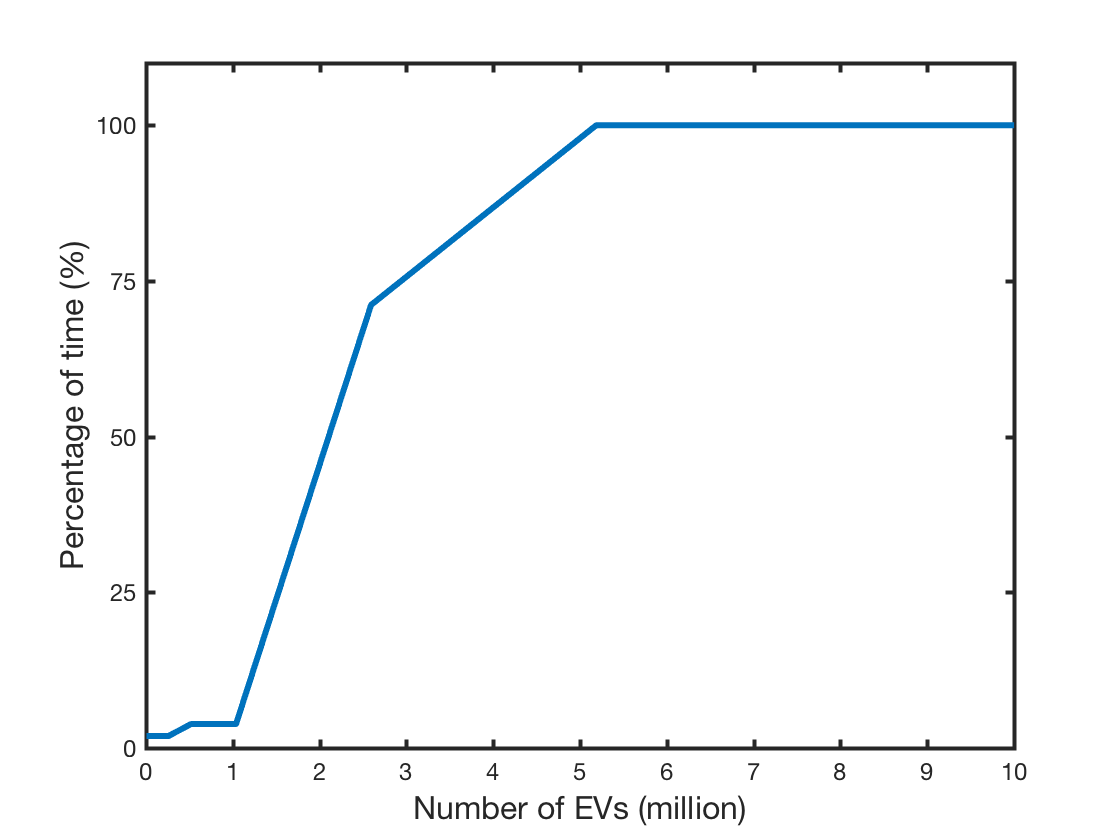
\includegraphics[width=0.95\linewidth]{Figures/EV_nan_percentage}
	\caption{Percentage of time when EV charging demand cannot be fulfilled in Germany}
	\label{fig:EV_nan_percentageg}
\end{figure}

This finding implies when there will be 1 million more EVs in Germany compared to the number in 2016, it will create great incentives for infrastructure extension of electricity grid, which reveals a promising business opportunity. Nevertheless, studies under that condition is beyond the focus of our work. Instead, we would only perform scenario analysis when the number of EV is within the limit of 1 million. 

In this thesis, we applied three scenarios studying the EV2G market in Germany:

\begin{itemize}
	\item \textbf{EV number 2016:} assuming all  EVs in Germany by 2016 are contract for delivering EV2G services
	\item \textbf{EV number 2017:} similar to the first scenario but using the data of 2017
	\item \textbf{2\% market share:} assuming EVs will account for 2\% of the total vehicle number in Germany (45 million according to \cite{Eurostat_de_v}) i.e. 0.9 million EVs in the future
\end{itemize}

According to the Federal Motor Transport Authority of Germany (Kraftfahrt-Bundesamtes, KBA)\cite{KBA2017}, the number of plug-in electric vehicles has grown fast over the past year, especially in 2017. Since the EV registered before 2010 is negligible, we conceived the cumulative registration since 2010 as the total number of EVs in Germany, shown as Figure \ref{fig:Germany_EV_number}.

\begin{figure}[h!]
	\centering
	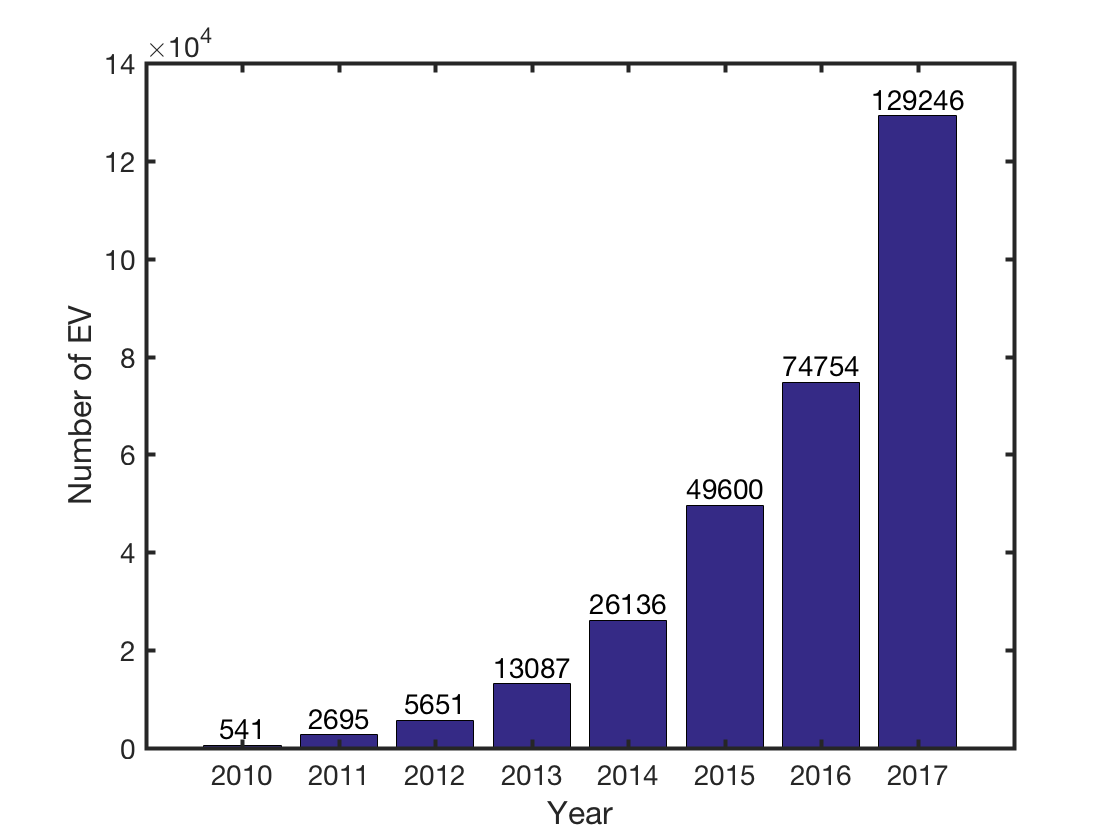
\includegraphics[width=0.95\linewidth]{Figures/Germany_EV_number}
	\caption{Cumulative registration of plug-in electric vehicles in Germany since 2010 \cite{KBA2017}}
	\label{fig:Germany_EV_number}
\end{figure}

The numbers of EV that were taken for the scenario analysis are then determined and list in Table \ref{tab:ev-number-scenario-germany}.

\begin{table}[h!]
	\centering
	\begin{tabular}{l r r}
		\hline
		\textbf{Scenario} & \textbf{EV number total} & \textbf{EV number per household} \\
		%\hline
		\hline
		EV number 2016 &  \num{74754} & \num{0.014} \\
		EV number 2017 &  \num{129246} & \num{0.025} \\
		2\% market share &  \num{900000} & \num{0.174} \\
		\hline
	\end{tabular}
\caption{The number of EV for each scenario in Germany}\label{tab:ev-number-scenario-germany}
\end{table}

\begin{figure}[h!]
	\centering
	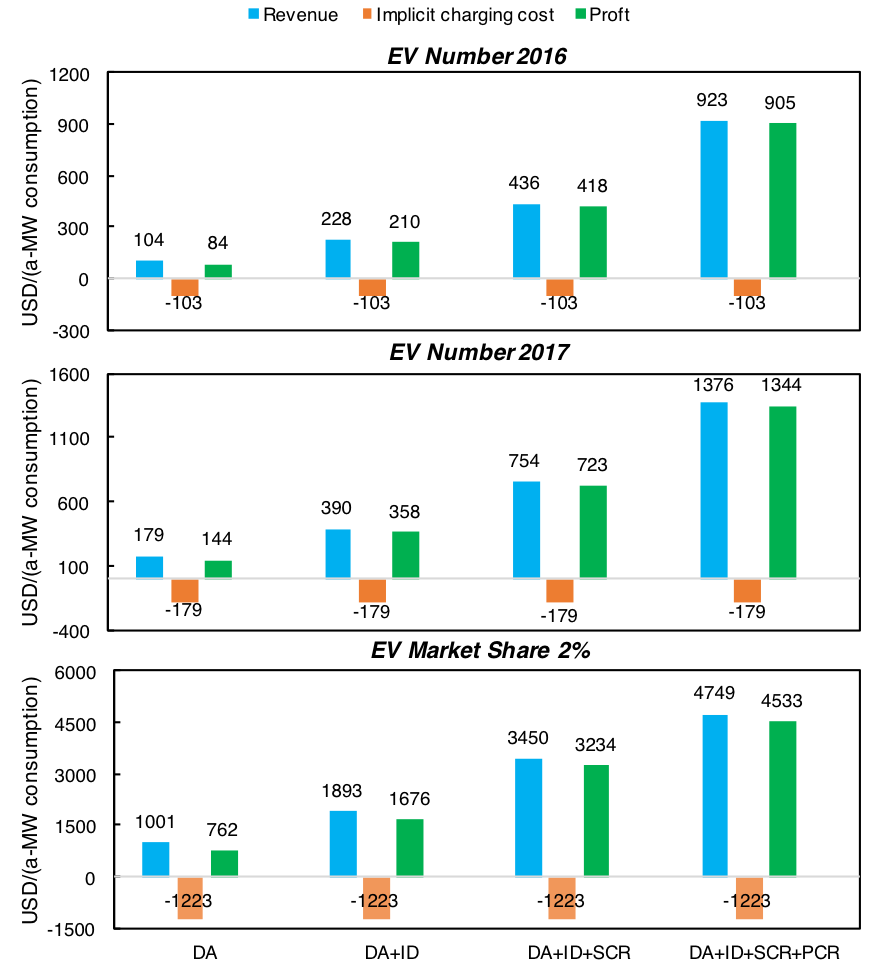
\includegraphics[width=0.95\linewidth]{Figures/Germany_EV_profit}
	\caption{Market size and profitability of EV2G in Germany electricity markets}
	\label{fig:Germany_EV}
\end{figure}

Based on these scenarios, we performed the case studies and the results are shown by Figure \ref{fig:Germany_EV}. It was found that the arbitrage only in day-ahead market was not profitable at all, while arbitrage in both day-ahead and intra-day market was barely able to maintain a revenue-cost balance. The revenues captured from arbitrage was at most compensating the cost of EV charging. Profits would be possible if a business model where services providers could charge service fees from the end-users (EV owners). Although the service fees can be much lower than the normal charging costs for the end-consumers, it would be still challenging in practice to implement such a business model because the charging cost become implicitly embedded when a EV was used for V2G services. Overall, the low arbitrage values in Germany's energy market makes these business cases not appealing. 

Coupling frequency control markets increases indeed the profits and it was found to be more promising with the drastic of EVs as there are still much more growth space till the scenario of 2\% EV market share. However, it shall be noticed that our analysis has overlooked some factors which could make the business less profitable as shown here. The main issue is that we use a determinate approach to simulate the frequency control signal and EV driving behaviors which eliminated the risks of failing to deliver the frequency control services as planned. Alipour \textit{et. al.}\cite{Alipour2017} made a study on EV2G for frequency control services with a stochastic approach. It was found in a case where a profit of 7980 USD was expected, the conditional value-at-risk was 5720 USD, indicating the risking nature of such a business. In the outlook of this thesis, we proposed a stochastic method by using Markov chain to simulate the uncertain driving behavior of EVs and then the estimation of risk can be conducted. Nonetheless, while quantitative risk assessment against uncertainty is necessary for designing a specific project, it is beyond the focus of a study understanding the whole market value so is not included in our study. Besides, implementing EV2G for frequency control is not a mature technology due to its complexity\cite{Peng2017}\cite{Shafie-Khah2015}\cite{Bessa2014}\cite{Bessa2013}, which implies a high research and development cost.

It is also worthwhile to note that while the number of EVs (0.9 million ) in the scenario of ``2\% Market Share" has reached the edge of the affordable level (1 million) for the grid, revenues are significantly smaller than the maximum potential revenues derived in the case studies of ESSs. The shares of maximum achievable revenue by EV2G to the total market potential by generic ESS were between 18-37\% among different cases. This reveals that constrained by the limitations discussed above, EV2G will not be able fully cover the needs for flexibility by its own, even on a aggregated system level without considering the distributed manners. Other types of flexibility would still be necessary to complement the demands for flexibility in scenarios with high EV penetrations.

\subsubsection{EV2G in PJM: RegD market would be saturated shortly if EV2G was indeed implemented}

\begin{figure}[h!]
	\centering
	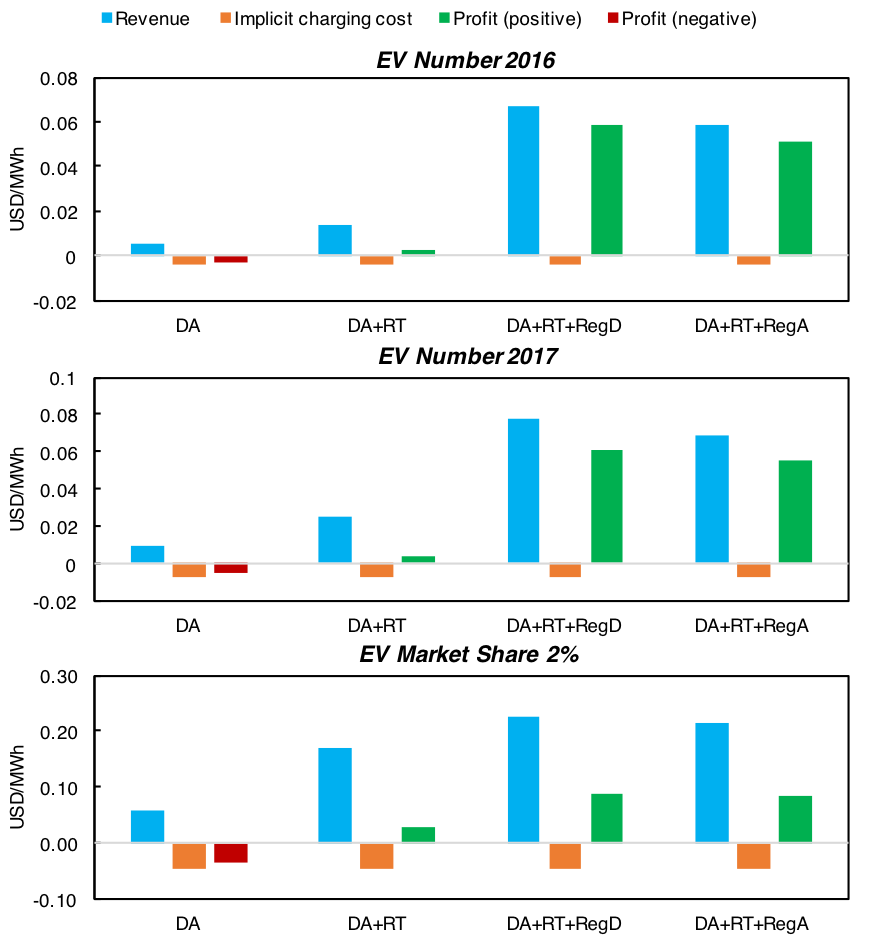
\includegraphics[width=0.95\linewidth]{Figures/PJM_EV_profit}
	\caption{Market size and profitability of EV2G in PJM Electricity markets}
	\label{fig:PJM_EV}
\end{figure}

Similar studies are performed in PJM power markets. Since the geographic coverage of PJM is not strictly corresponding to the administrative divisions, it becomes a extremely sophisticated task to get the official number of EVs in PJM with the public data. Therefore, we projected the number in Germany to PJM by their ratio of household number. That means, in the corresponding scenarios, the EV ownership per household is identical in Germany and PJM. We took this approach to make an indication of the market value, which however shall be noticed with caution that it may deviate from real conditions. 
Table \ref{tab:ev-number-scenario-PJM} shows the number of EV in each scenario.

\begin{table}
	\centering
	\begin{tabular}{ l r r }
		\hline
		\textbf{Scenario} & \textbf{EV number total} & \textbf{EV number per household} \\
		%\hline
		\hline
		EV number 2016 &  \num{43713} & \num{0.014} \\
		EV number 2017 &  \num{75578} & \num{0.025} \\
		2\% market share &  \num{526290} & \num{0.174} \\
		\hline
	\end{tabular}
	\caption{The number of EV for each scenario in PJM}\label{tab:ev-number-scenario-PJM}
\end{table}

With these numbers of EV, no generation shortage was observed, expect for only one week in the scenario of 2\% EV market share. The results in that week were discarded, i.e. no operations and thus no revenues in that week. This accounts for approximately 2\% of the time in a year so the impact on final results shall be negligible.

Figure \ref{fig:PJM_EV} summarizes the results of cases in PJM. Arbitrage in day-ahead market only was still not profitable. Coupled operations in real-time market lead to niche profits while the EV numbers are relative small, which is similar to the situation in Germany. However, with a 2\% EV market share, we saw a profit from business case while it incurred loss in Germany's DA+ID markets. This can be explained by the PJM's real-time market as a hub for all real-time settlements has much higher liquidity than the intra-day exchange in Germany.

The incremental revenue by stacking RegD to DA+RT case was 462 USD/$(\text{a} \cdot \text{MW})$ in the scenario of ``EV Number 2016" while the addtional revenue by stacking SCR to DA+ID in Germany was merely 206 USD/$(\text{a} \cdot \text{MW})$, which again reveals the favor of RegD toward flexibility resources. 

Noticing that the whole RegD market potential for generic flexiblity resources is merely 513 USD/$(\text{a} \cdot \text{MW})$ as was shown previously by \ref{fig:pjm-ess}. This market could be easily exhausted by a small size of EV fleet. 
 
\subsubsection{EV2G in NSW: arbitrage-only is more profitable than frequency control in the other two geographies}

Using the same methodology as in PJM, scenarios are established by taking the identical EV numbers per household, as is shown by Table \ref{tab:ev-number-scenario-nsw}. With these number of EV, no supply shortage was observed.  

\begin{table}[h!]
	\centering
	\begin{tabular}{ l r r }
		\hline
		\textbf{Scenario} & \textbf{EV number total} & \textbf{EV number per household} \\
		%\hline
		\hline
		EV number 2016 &  \num{4849} & \num{0.014} \\
		EV number 2017 &  \num{8383} & \num{0.025} \\
		2\% market share &  \num{58377} & \num{0.174} \\
		\hline
	\end{tabular}
	\caption{The number of EV for each scenario in NSW}\label{tab:ev-number-scenario-nsw}
\end{table}

\begin{figure}[h!]
	\centering
	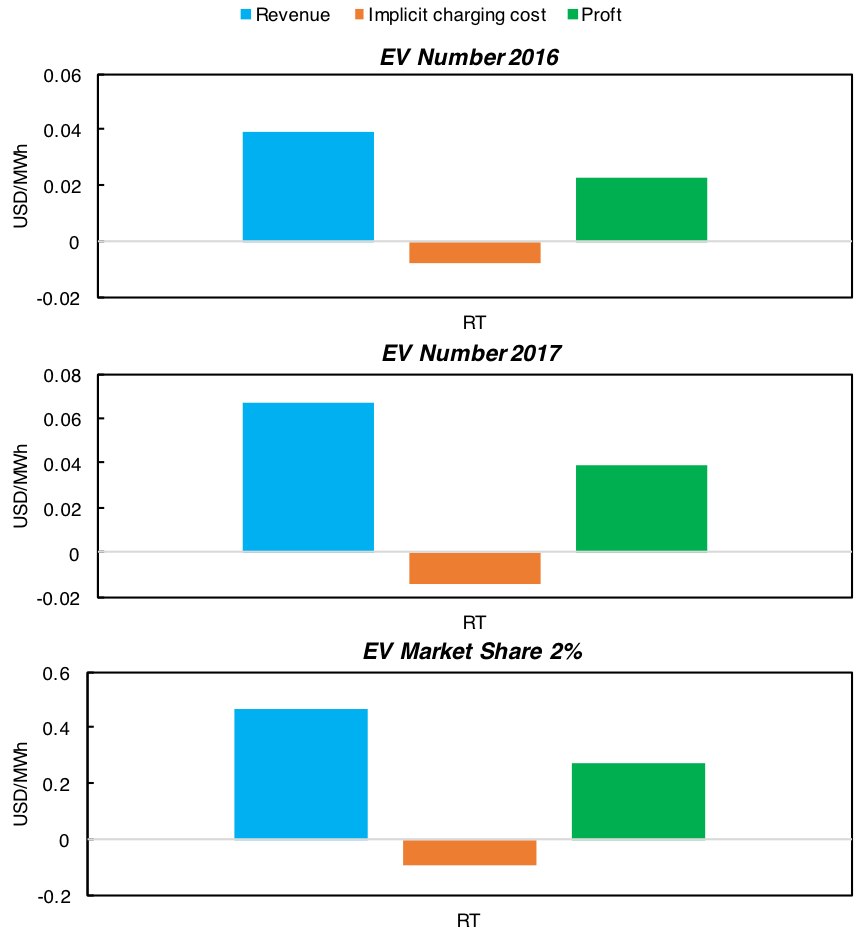
\includegraphics[width=0.95\linewidth]{Figures/NSW_EV_profit}
	\caption{Market size and profitability of EV2G in NSW Electricity markets}
	\label{fig:NSW_EV}
\end{figure}

Figure \ref{fig:NSW_EV} presents the results of three scenarios in NSW's real-time energy market. Similar to the situations in ESS cases, the market potential of arbitrage is higher than the other two geographies due to the price volatility as is cussed previously. The potential profit obtained in the scenario of ``EV Number 2016" was \num{198} USD/$(\text{a} \cdot \text{MW})$, which was 66 and 9 times the numbers in corresponding cases in Germany and PJM respectively. It is even higher than profits from business cases where frequency control are involved in other two geographies. Since arbitrage using EV is much more feasible in technology, such a high arbitrage profitability shall provide more incentives for the market participates and makes the business appealing if the number of EV will indeed grow in line with our scenarios.

Finally, it shall be noted that even in the scenario with 2\% EV market share, the market potential of arbitrage via EV2G was found to be \num{4105} USD/$(\text{a} \cdot \text{MW})$, which was just 3.8\% of the overall arbitrage potential using ample size of generic ESSs as was shown by Figure \ref{fig:nsw-ess}, leaving a vast space for other technologies.

\subsubsection{Summary}

The key indicators for the market size and profitability, in both normalized and absolute values are summarized in Table \ref{tab:germany-summary}-\ref{tab:nsw-summary}. Values were extracted at different scenarios where they are maximized. Therefore, the maximum revenue and maximum profit may not be obtained at the same time, especially for ESSs, as has been discussed at the beginning of this section.

\begin{table}
	\centering
	\begin{tabular}{l r r r r}
		\hline
		\multirow{2}{*}{\textbf{Item\footnote{Maximum values of items are obtained in different scenarios}}}& \textbf{Arbitrage} & \multicolumn{2}{c}{\textbf{Balancing}} & \textbf{Multitasking} \\
		\multirow{2}{*}{}& DA+ID & BE & FCR\footnote{Frequency control reserve, including both PCR and SCR} & DA+ID+FCR \\
		\hline
		\multicolumn{5}{l}{\textbf{Energy Storage System}} \\
		& & & & \\
		Max. Revenue [USD/$(\text{a} \cdot \text{MW})$] & \num{6426} & \num{3872} & \num{2012} & \num{10247} \\
		Max. Profit [USD/$(\text{a} \cdot \text{MW})$] & - & 17 & - & - \\
		& & & & \\
		Max. Revenue [mUSD/a] & \num{380} & \num{229} & \num{119} & \num{606} \\
		Max. Profit [mUSD/a] & - & 1 & - & - \\
		& & & & \\
		Max. Profitability Ratio & (-92\%) & 7\% & (-40\%) & (-60\%) \\
		Cost break-even\footnote{Cost reduction ratio} & (-84\%) & - &- & -\\
		& & & &\\
		\hline
		\multicolumn{5}{l}{\textbf{Electric Vehicle to Grid}} \\
		& & & & \\
		Max. Revenue [USD/$(\text{a} \cdot \text{MW})$] & \num{1961} & - & - & \num{3224} \\
		Max. Profit [USD/$(\text{a} \cdot \text{MW})$] & 8 & - & - & \num{1986} \\
		& & & & \\
		Max. Revenue [mUSD/a] & \num{116} & - & \- & \num{190} \\
		Max. Profit [mUSD/a] & \num{0.5} & - & - & 117 \\
		& & & & \\
		Max. Profit per EV [USD/(a)] & \num{4} & - & - & \num{731} \\
		& & & &\\
		\hline
	\end{tabular}
	\caption{Summary of market size and profitability of flexibility management in Germany}\label{tab:germany-summary}
\end{table}

\begin{table}
	\centering
	\begin{tabular}{l r r r r}
		\hline
		\multirow{2}{*}{\textbf{Item\footnote{Maximum values of items are obtained in different scenarios}}}& \textbf{Arbitrage} & \multicolumn{2}{c}{\textbf{Balancing}} & \textbf{Multitasking} \\
		\multirow{2}{*}{}& DA+RT & RegD & RegA & DA+RT+Reg\footnote{Including both RegD and RegA}\\
		\hline
		\multicolumn{5}{l}{\textbf{Energy Storage System}} \\
		& & & & \\
		Max. Revenue [USD/$(\text{a} \cdot \text{MW})$] & \num{6333} & \num{524} & \num{467} & \num{7324} \\
		Max. Profit [USD/$(\text{a} \cdot \text{MW})$] & 0 & 11 & 0 & 53\\
		& & & &\\
		Max. Revenue [mUSD/a] & \num{556} & \num{46} & \num{41} & \num{643}\\
		Max. Profit [mUSD/a] & 0 & 1 & 0 & 3\\
		& & & & \\
		Max. Profitability Ratio & (-88\%) & 8\% & (-29\%) & 9\%\\
		Cost break-even\footnote{Cost reduction ratio} & (-81\%) & - & - & -\\
		& & & & \\
		\hline
		\multicolumn{5}{l}{\textbf{Electric Vehicle to Grid}} \\
		& & & & \\
		Max. Revenue [USD/$(\text{a} \cdot \text{MW})$] & \num{1504} & - &  - & \num{2351}\\
		Max. Profit [USD/$(\text{a} \cdot \text{MW})$] & 261 & - & - & \num{1218} \\
		& & & & \\
		Max. Revenue [mUSD/a] & \num{132} & - &  - & \num{206}\\
		Max. Profit [mUSD/a] & \num{23} & - &  - & \num{107} \\
		& & &  & \\
		Max. Profit per EV [USD/(a)] & \num{45} & - & - &\num{1657}\\
		& & & & \\
		\hline
	\end{tabular}
	\caption{Summary of market size and profitability of flexibility management in PJM}\label{tab:pjm-summary}
\end{table}

\begin{table}
	\centering
	\begin{tabular}{l r r}
		\hline
		\multirow{2}{*}{\textbf{Item\footnote{Maximum values of items are obtained in different scenarios}}}& \textbf{Arbitrage} & \textbf{Balancing} \\
		\multirow{2}{*}{}& DA+RT & FCAS\footnote{Values based on payment on a whole system level without involving technical analysis} \\
		\hline
		\multicolumn{3}{l}{\textbf{Energy Storage System}} \\
		& & \\
		Max. Revenue [USD/$(\text{a} \cdot \text{MW})$] & \num{109301} & \num{2933} \\
		Max. Profit [USD/$(\text{a} \cdot \text{MW})$] & - & - \\
		& & \\
		Max. Revenue [mUSD/a] & \num{872} & \num{23} \\
		Max. Profit [mUSD/a] & - & - \\
		& & \\
		Max. Profitability Ratio & (-70\%) & - \\
		Cost break-even\footnote{Cost reduction ratio} & (-68\%) & \\
		& & \\
		\hline
		\multicolumn{3}{l}{\textbf{Energy Storage System}} \\
		& & \\
		Max. Revenue [USD/$(\text{a} \cdot \text{MW})$] & \num{4105} & - \\
		Max. Profit [USD/$(\text{a} \cdot \text{MW})$] & \num{2382} & - \\
		& & \\
		Max. Revenue [mUSD/a] & \num{33} & - \\
		Max. Profit [mUSD/a] & 19 & - \\
		& & \\
		Max. Profit per EV [mUSD/a]& 326 & - \\
		& & \\
		\hline
	\end{tabular}
	\caption{Summary of market size and profitability of flexibility management in NSW}\label{tab:nsw-summary}
\end{table}

\newpage
\subsection{Impact analysis of renewable penetration}
\label{sec:impact-market-condition}

As is mentioned at the beginning of this section, understanding the impact of some key factors is crucially viable to plan future business on flexibility management, as the market may evolve rapidly. Among all the factors, we have selected the renewable penetration as the most influencing factor and studied in this thesis. The rationale can be explained as the renewable penetration would change most radically compared to other factors and is viewed as the essential driver of growing needs for flexibility, which has been elaborated in Chapter \ref{ch:introduction}. 

Growing capacity of renewable generations will influence both wholesale energy and frequency control markets as we have seen from the literature; refer to Chapter \ref{ch:LitRev}. However, determining the requirement for frequency control reserve is an extremely sophisticate process of grid planning, which is rarely addressed by academic articles. Grid planner may initiated large-scale research project dealing with this problem. Referring to a study ordered by PJM and conducted by a research consortium led by GE Consulting\cite{GEEnergyConsulting2014}, an average of 1533 MW frequency regulation reserve would be required in a scenario where the 14\% RPS (Renewable Portfolio Standard by each state in PJM region) is to be met by 2026. This is about 2.2 times of the amount in 2016 (700MW). Assuming the price stays at the same level, one may multiply the ratio of 2.2 to the valuation results presented in preceding section, in order to make a rough estimation of the future. Nonetheless, the penetration of renewable will not only influence the frequency control market physically but also institutionally where the design of market may be revised. Therefore, understanding quantitatively the impacts of renewables on both volume and price in frequency control market are significantly beyond the scope of this study. 

In this thesis, we would only focus on the wholesale energy market. Day-head markets in both Germany and PJM are taken for case studies.

In order to simulate price scenarios with different level of renewable generation, we adopted a simplified method by multiplying the time-series data of actual renewable generation in 2016 by a certain ratio. No simulations with wealth data were involved. 

In Germany, the installed capacity of solar and wind has already accounted for a significant share, i.e. \num{83.85} GW as 41.7\% of the total generation capacity. Therefore, we made conservative scenarios where the assumed capacity of wind and solar are 85\% to 115\% of present level with a step length of 5\% of the existing capacity, equal to 4.19 GW per step. 

%\num{105870 } GWh 2016 in Germany, including both wind and solar generations. Therefore, a change of 5\% in renewable generation can be deemed as equivalent to 4.19 GW or \num{8.29} GWh. 


For PJM, the installed capacity of wind and solar was merely 6533 MW in 2016, which is 3.7\% of the total capacity. The 14\% RPS, as is mentioned above, requires PJM to install a total of \num{40190} MW solar and wind generations by 2026. Compared to the number in 2016, this indicates a compound annual growth rate (CAGR) of 20\%. Therefore, we created additional scenarios beyond the ones that are consistent with German cases (85-115\%) as 5-year forecasts the 20\% CAGR.

\subsubsection{Model setup and validation}
In order to analyze the future trend of market value by understanding potential impacts of certain key factors, the market simulation module was designed as is introduced in Section \ref{sec:market-simulation}. In this section, we would demonstrate the setup and validation of the module  based on day-ahead market and generation data in Germany in 2016.

First of all, the data of Germany day-ahead price and volume were collected and shown as Figure \ref{fig:merit-orignal}.

\begin{figure}[h!]
	\centering
	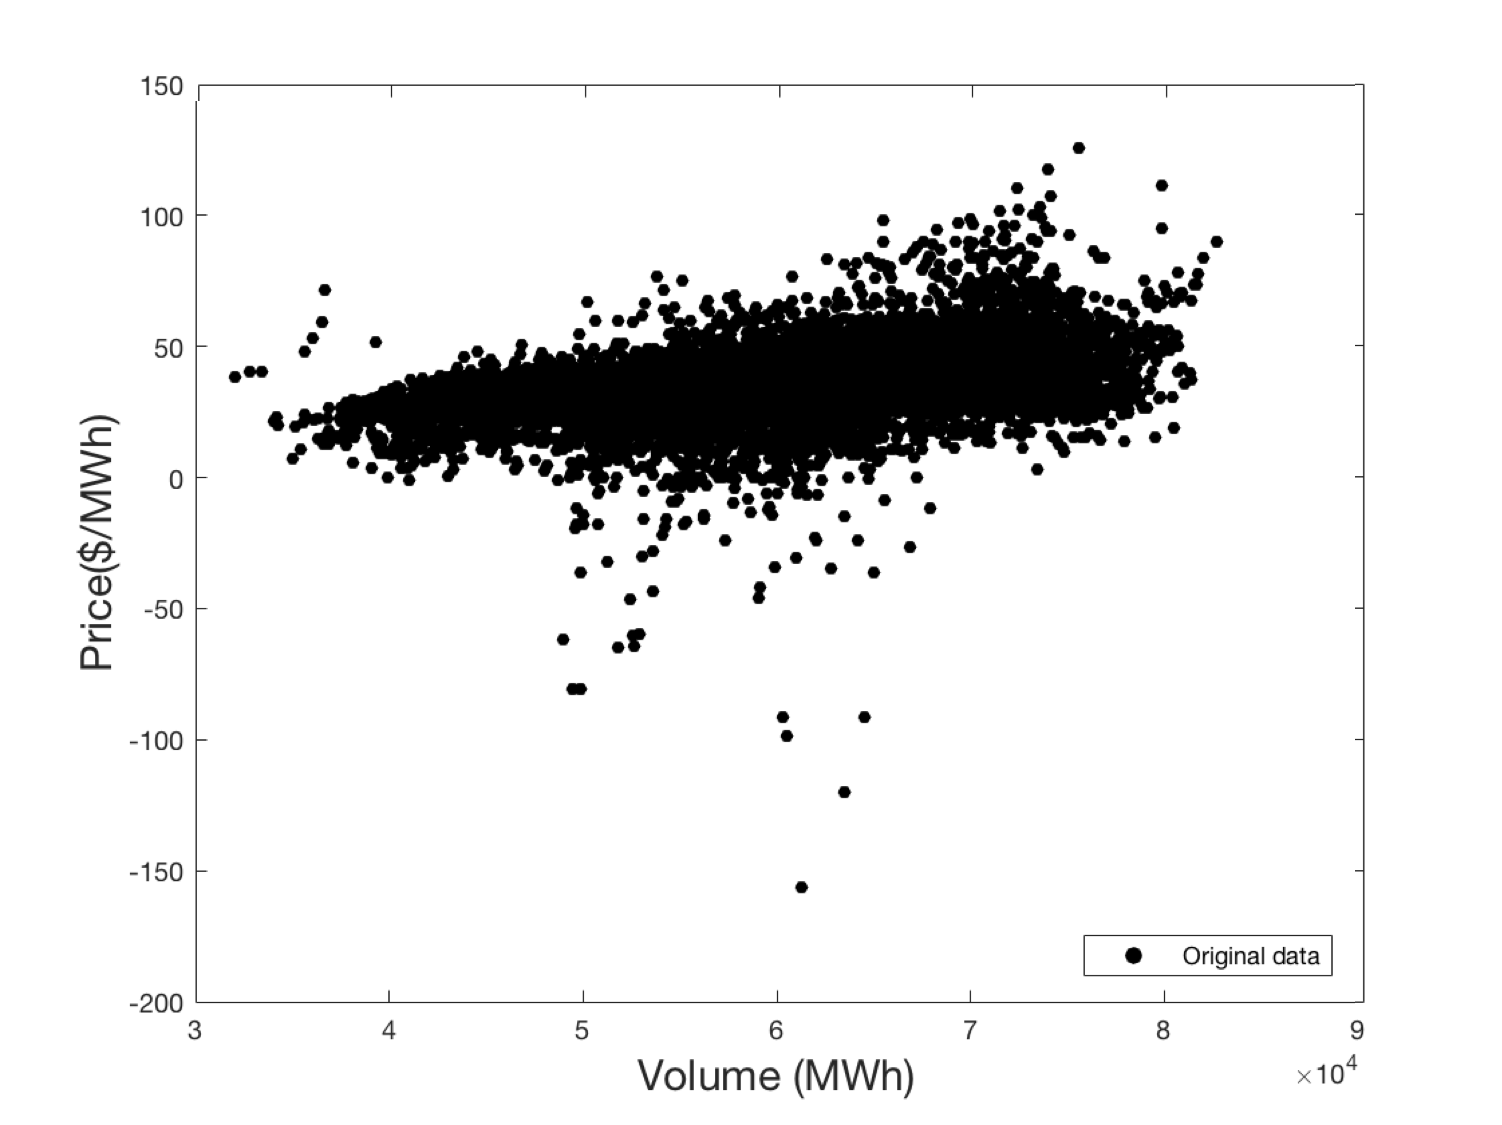
\includegraphics[width=0.95\linewidth]{Figures/Merit-order-original}
	\caption{Germany day-ahead price-volume data in 2016}
	\label{fig:merit-orignal}
\end{figure}

The pattern of merit-order effect is not clearly recognizable from the original data mainly due to the disturbs of variable renewable generation which has raised significantly in past years. This prevents us from directly applying merit-order models developed by previous studies\cite{He2013}\cite{Grunewald2012a}. Therefore, we applied the algorithm described in Section \ref{sec:market-simulation} which take into account the renewable generation and bounded flexibility of conventional generations. Figure \ref{fig:merit-transformed} shows the transformed pattern of data where a clearer merit-effect is identifiable. Figure \ref{fig:merit-classified} projects the classification to the original data distribution and it can be seen that the algorithm has successfully separated the data points where the price was driven to be higher or lower than average level due to the uplift effects introduced in \ref{sec:market-simulation}. 

\begin{figure}[h!]
	\centering
	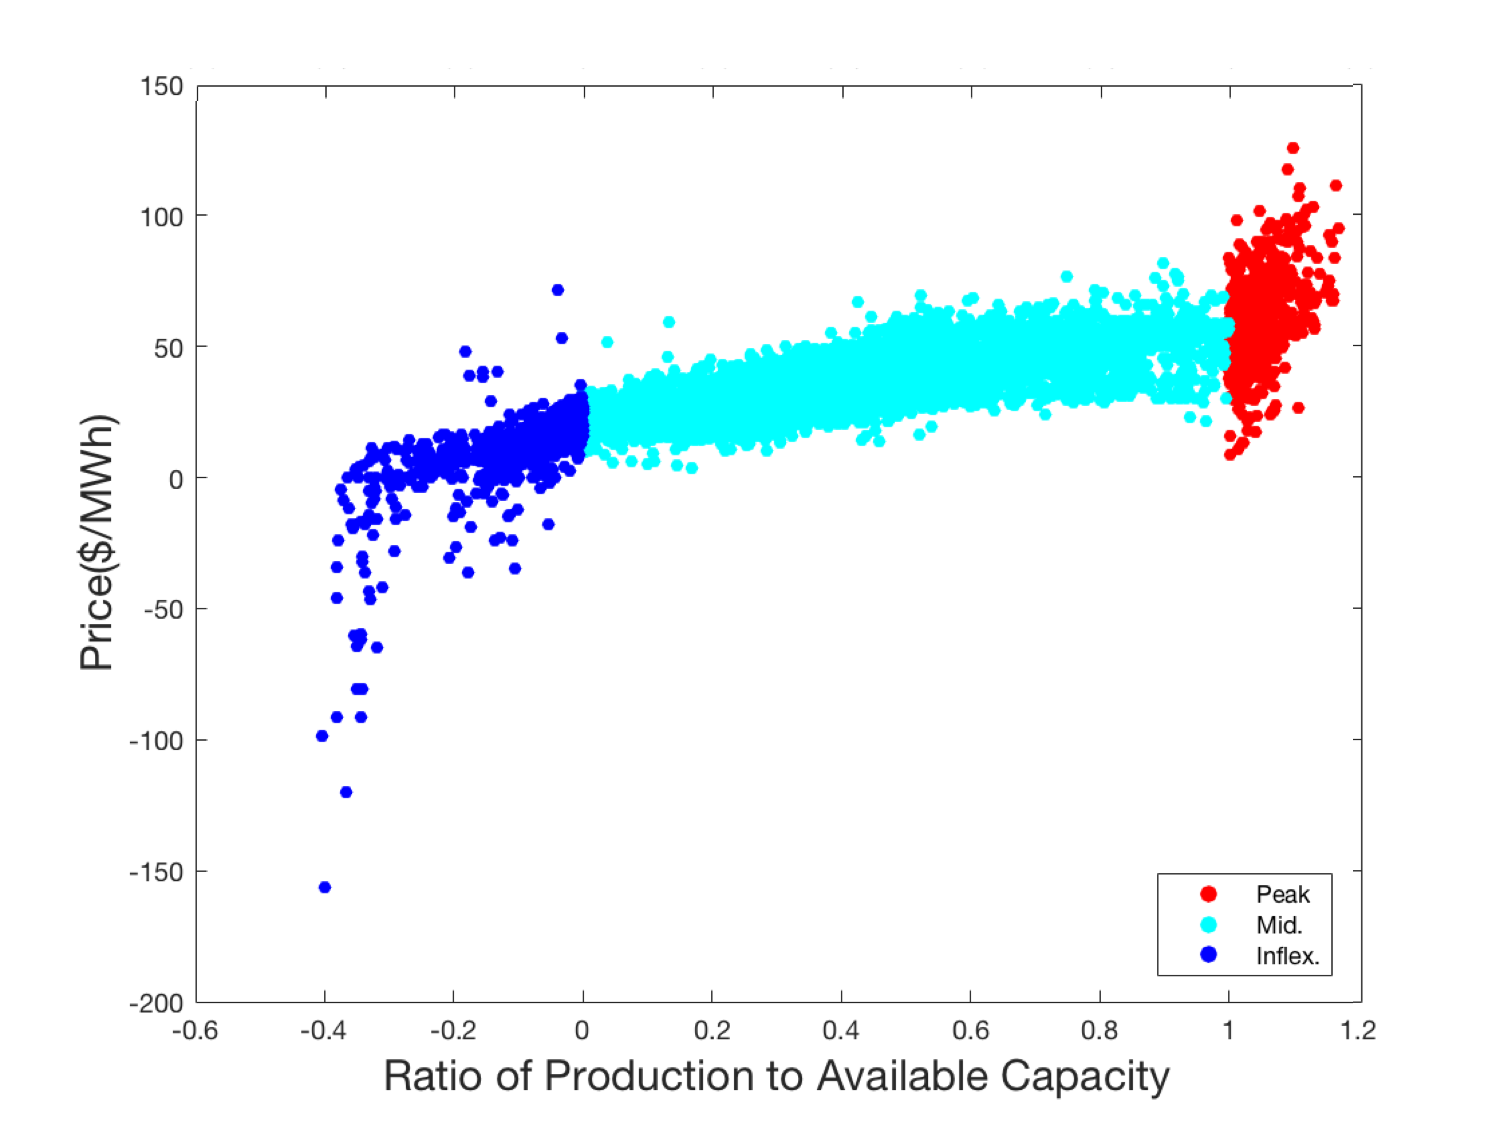
\includegraphics[width=0.95\linewidth]{Figures/Merit-order-transformed}
	\caption{Transformed pattern of Germany day-ahead price-volume data in 2016}
	\label{fig:merit-transformed}
\end{figure}
\begin{figure}[h!]
	\centering
	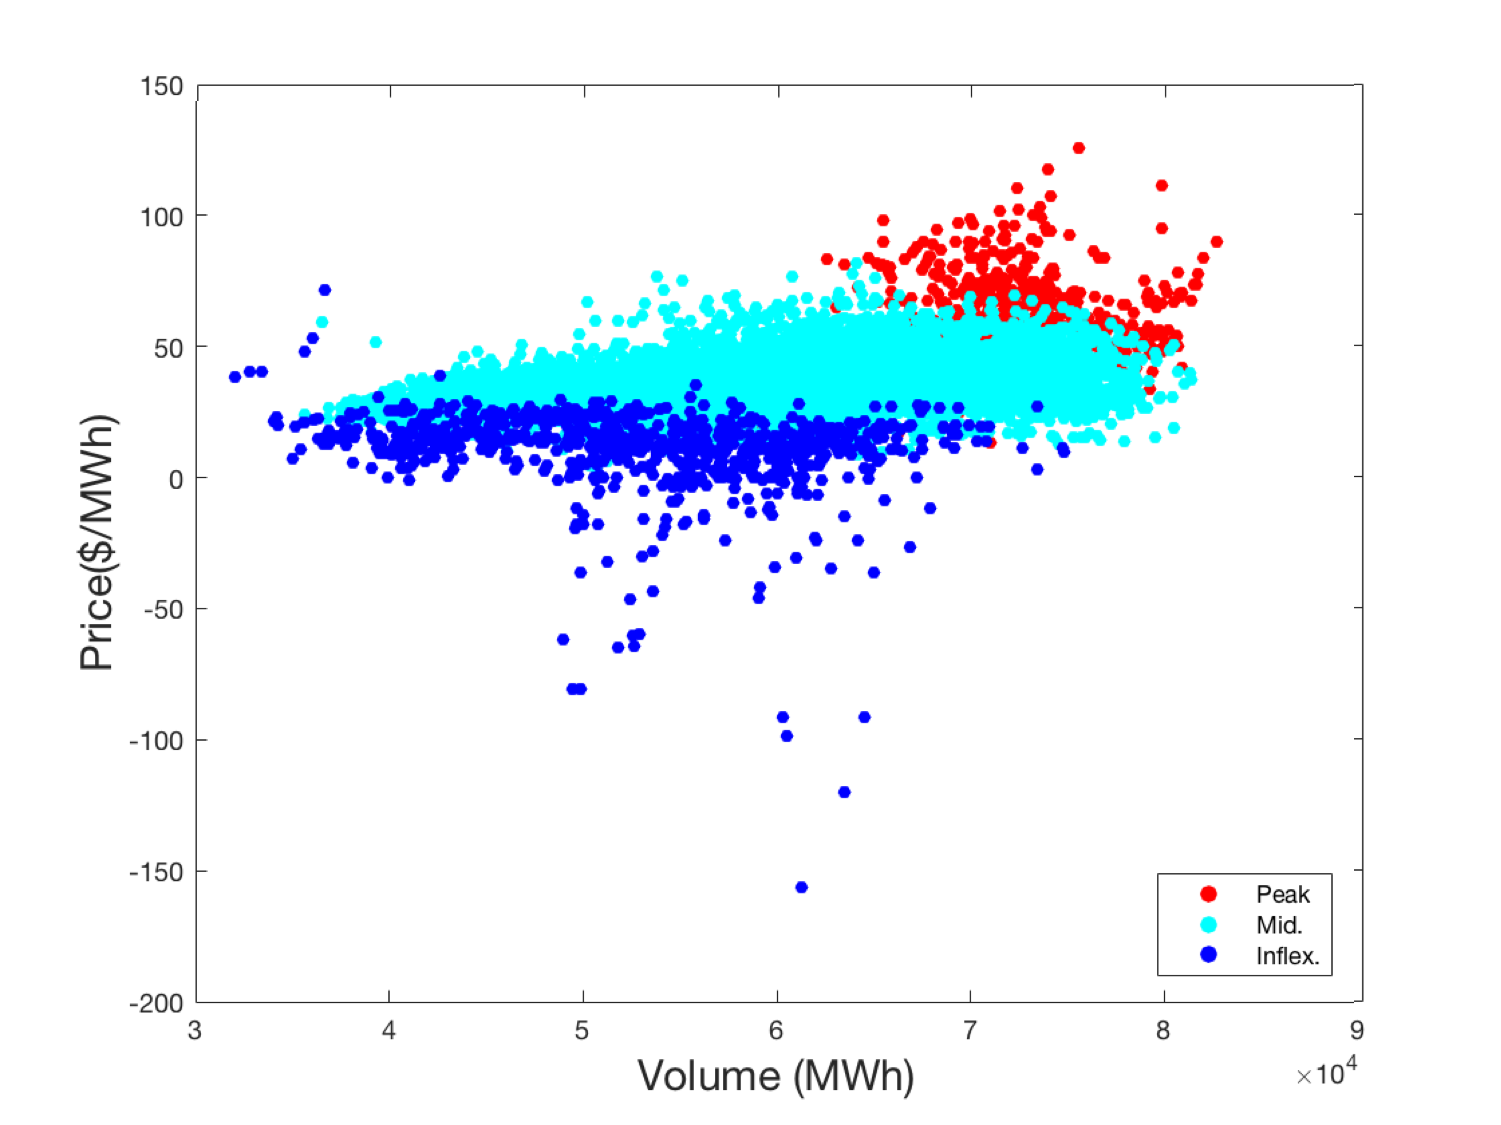
\includegraphics[width=0.95\linewidth]{Figures/Merit-order-classified}
	\caption{Classification of Germany day-ahead price-volume data in 2016}
	\label{fig:merit-classified}
\end{figure}

Thereafter, we fitted the transformed data pattern with the piece-wise function defined by \eqref{eq:merit-order-model}. The estimated parameters are listed in Table \ref{tab:merit}. It shall be noticed there are price limits applied in EPEX day-ahead market\cite{EPEX_price_limit} which is between -500 to 3000 EUR/MWh, equal to -600 to 3.6 USD/MWh using the specified currency exchange rate. The fitted merit-order curve is illustrated by Figure \ref{fig:merit-fitted} and distribution of errors between the fitted price and actual price is shown by Figure \ref{fig:merit-error}.

\begin{table}[h!]
	\centering
	\begin{tabular}{l  r r r}
		\hline
		\multirow{2}{*}{\textbf{Class}} & \multicolumn{3}{c}{\textbf{Parameters}}\\
		 & $a$ & $b$ & $c$\\
		\hline
		Inflex. & 17.05 & 1.49 & 12.35 \\
		\multirow{3}{*}{Mid.} & 48.66 & 16.40 & \\
		\multirow{3}{*}{} & 38.04 & 20.12 & \\
		\multirow{3}{*}{} & 16.37 & 34.20 & \\
		Peak & -194.95 & 491.46 & 0.69 \\
		\hline
	\end{tabular}
	\caption{Parameters of the merit-order model in Germany}\label{tab:merit}
\end{table}

\begin{figure}[h!]
	\centering
	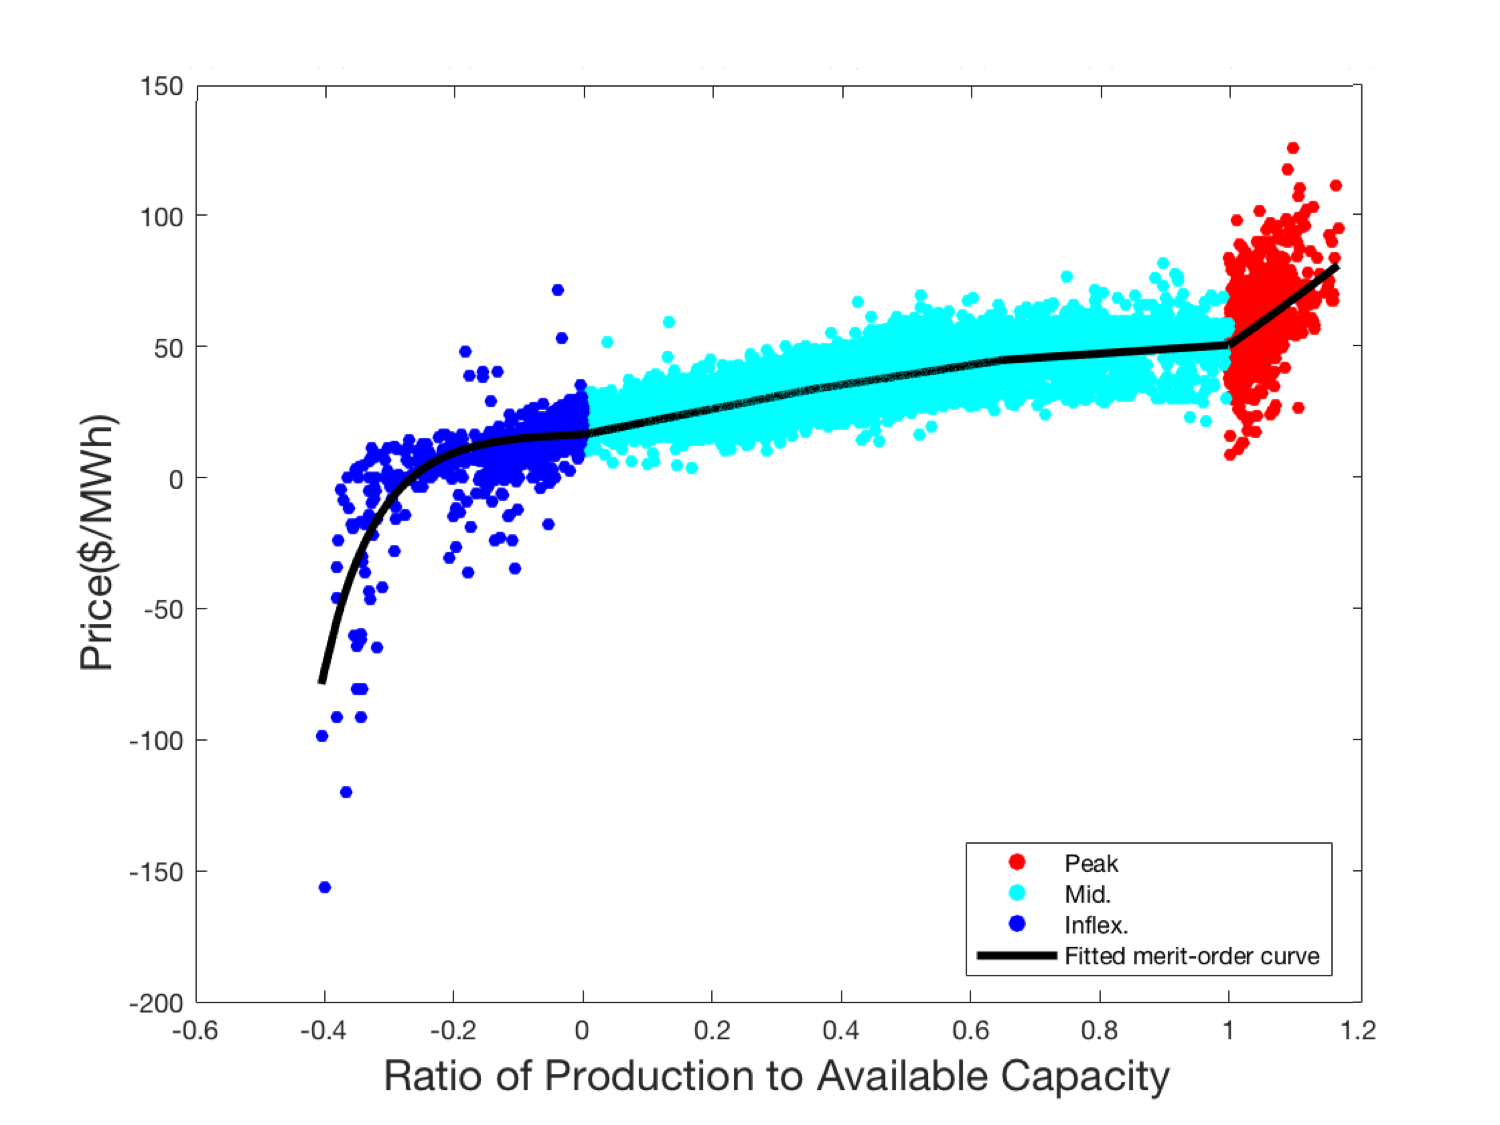
\includegraphics[width=0.95\linewidth]{Figures/Merit-order-fitted}
	\caption{Fitted merit-order curve with Germany day-ahead price-volume data in 2016}
	\label{fig:merit-fitted}
\end{figure}

\begin{figure}[h!]
	\centering
	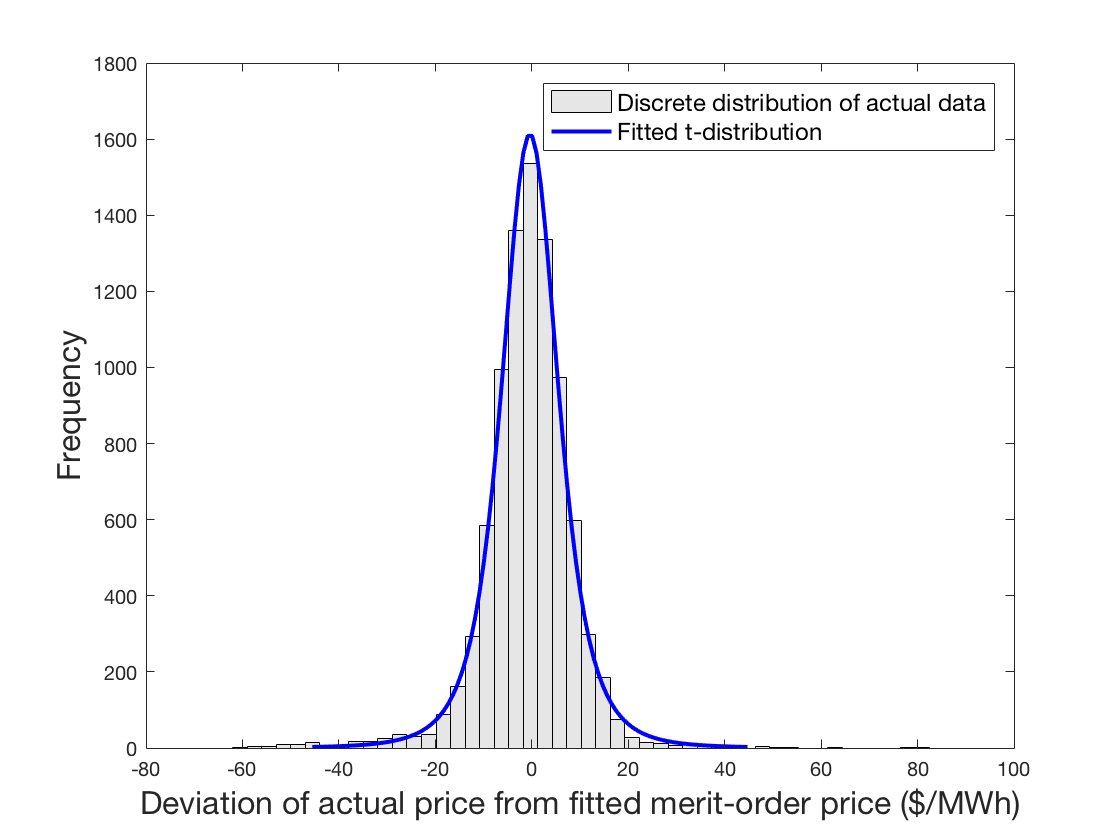
\includegraphics[width=0.9\linewidth]{Figures/4_Error-distribution}
	\caption{Distribution of errors between fitted merit-order price and actual price}
	\label{fig:merit-error}
\end{figure}

We simulated the day-ahead price using this merit-order model and compared to the actual market data. It can seen from Figure \ref{fig:merit-fitted}-\ref{fig:merit-error} that while the fitted merit-order price shows a good fitness to the actual price in terms of general trend, the stochastic movements of the price are eliminated. Merely with the merit-order model, a smoothed curve of price time-series would be generated where the drastic jumps of price cannot be captured, as is demonstrated by Figure \ref{fig:price-example}.

\begin{figure}[h!]
	\centering
	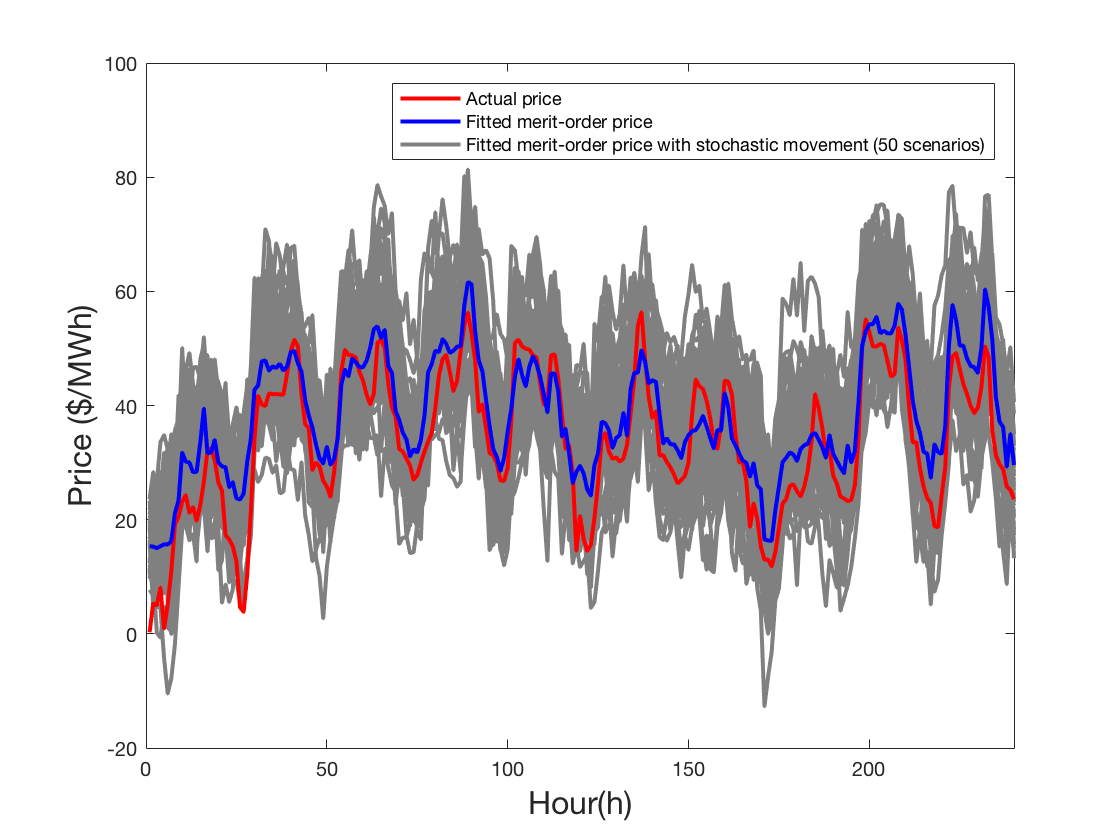
\includegraphics[width=0.95\linewidth]{Figures/5_Example-simulated_price}
	\caption{Generated price scenarios}
	\label{fig:price-example}
\end{figure}

Unlike studies on valuation of a conventional generation resources where such a merit-order model may suffice, the elimination of stochastic price movement would reduce the value of arbitrage greatly as is shown by Figure \ref{fig:model-validation}. This shall be understood intuitively as arbitrage activities pick the price differences among different trading slots and less volatile price movements would certainly affect the value creation of arbitrage.

\begin{figure}[h!]
	\centering
	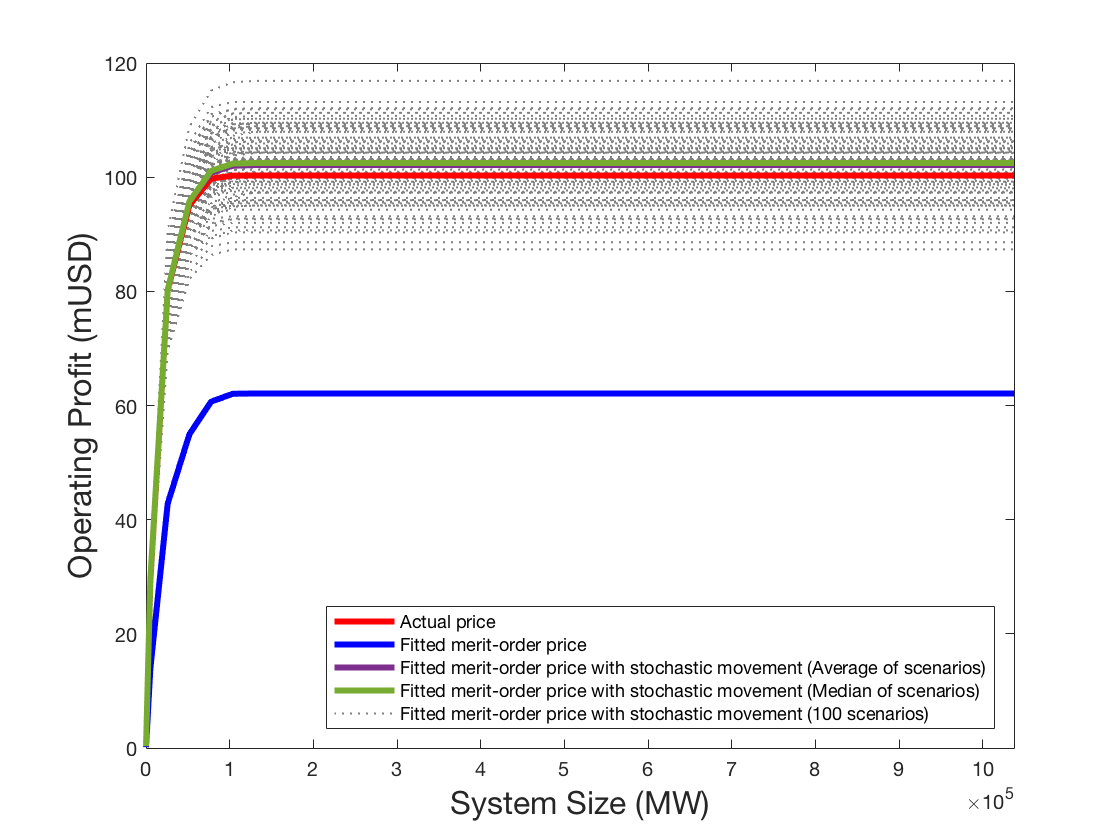
\includegraphics[width=0.95\linewidth]{Figures/6_Model_Validation}
	\caption{The revenue with different price scenarios for model validation in Germany}
	\label{fig:model-validation}
\end{figure}

\begin{table}[h!]
	\centering
	\begin{tabular}{r r}
		\hline
		\multicolumn{2}{c}{SARMA parameters}\\
		\hline
		$\omega_1 = 1.811$ & $\theta_1 = -1.063$ \\
		$\omega_2 = -0.813$ & $\theta_{24} =0.692$ \\
		$\omega_{24} = 0.090$ & $\theta_{168} = -0.600$ \\
		$\omega_{168} = 0.692$ & \\
		\hline
	\end{tabular}
	\caption{Parameters of the stochastic price movement of SARMA models in Germany}\label{tab:SARMA}
\end{table}

Therefore, a seasonal auto-regressed moving-average (SARMA) model as is described in \ref{sec:market-simulation} is applied to simulate the stochastic components of the price. The estimated parameters of the SARMA model based on the error signal characterized by\ref{fig:merit-error} is listed in Table \ref{tab:SARMA}. Thereafter, we conducted Monte-Carlo simulations and generated a number of scenarios of the stochastic parts of price which are then added to the determinate trends calculated by the merit-order model. The final simulated price scenarios are illustrated by the grey lines in Figure \ref{fig:price-example}. Using these generated price profiles, we calculated the revenue for 100 scenarios and compare the average and median value to the result obtained with actual price signal, which shew perfect fitness in Figure \ref{fig:model-validation}. There are no significant differences between the average and median value observed, but for robustness and avoiding effects of outliers, we would use the median value as the simulated result for experiments in proceeding sections.

We applied the same procedure to develop the model for PJM. It was noticed that the situation when the residual load is in the range of inflexible generation is rarely observed in PJM, which can be explained by the relative low installed capacity of renewable generations. Therefore, we migrated part of the merit-order model for inflexible generation based on Germany's data here, which shall however have insignificant effects because the lowest price is bounded at 0. Negative pricing is not explicitly an issue in PJM's market so far although PJM is fully aware of this issue but waiting for FERC's initiative to address the potential negative price formation\cite{PJM_price_limit_1}. Without unambiguous rules, we would not allow negative prices in our modeling. The highest price, on the other hand in PJM is capped at 1000 USD/MWh\cite{PJM_price_limit}. 

The parameters for the merit-order model in PJM are listed in Table \ref{tab:merit_pjm}. The SARMA parameters are presented in Table \ref{tab:SARMA_PJM}.

\begin{table}[h!]
	\centering
	\begin{tabular}{l  r r r}
		\hline
		\multirow{2}{*}{\textbf{Class}} & \multicolumn{3}{c}{\textbf{Parameters}}\\
		& $a$ & $b$ & $c$\\
		\hline
		Inflex. & 17.05 & 1.49 & 12.35 \\
		\multirow{3}{*}{Mid.} & 23.50 & 16.40 & \\
		\multirow{3}{*}{} & 32.02 & 13.41 & \\
		\multirow{3}{*}{} & 3.58 & 31.90 & \\
		Peak & 10.70 & 501.35 & 5.32 \\
		\hline
	\end{tabular}
	\caption{Parameters of the merit-order model in PJM}\label{tab:merit_pjm}
\end{table}

\begin{table}[h!]
	\centering
	\begin{tabular}{r r}
		\hline
		\multicolumn{2}{c}{SARMA parameters}\\
		\hline
		$\omega_1 = 0.690$ & $\theta_1 = 0.107$ \\
		$\omega_2 = 0.125$ & $\theta_{24} =-0.003$ \\
		$\omega_{24} = 0.298$ & $\theta_{168} = -0.399$ \\
		$\omega_{168} = 0.560$ & \\
		\hline
	\end{tabular}
	\caption{Parameters of the stochastic price movement of SARMA models in PJM}\label{tab:SARMA_PJM}
\end{table}


\subsubsection{Renewable penetration in Germany: at the inflection point}


\begin{figure}[h!]
	\centering
	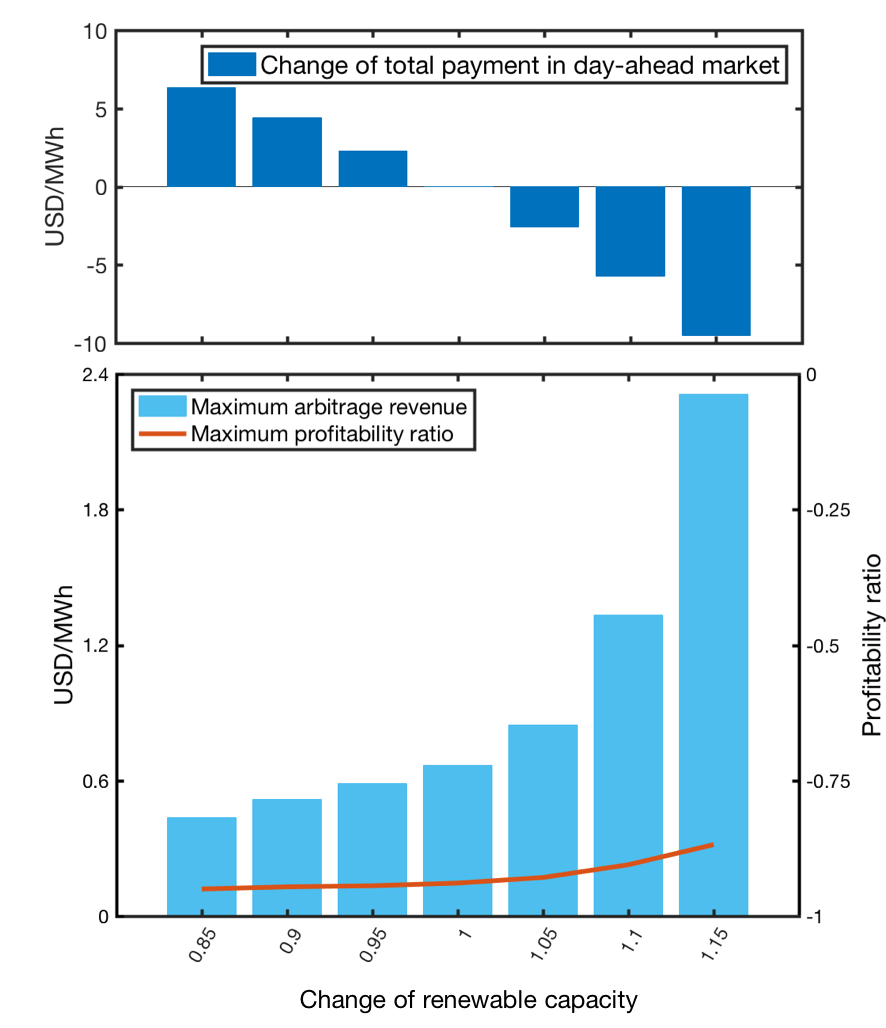
\includegraphics[width=0.95\linewidth]{Figures/RenewablePenetration_Germany}
	\caption{Impacts of renewable generations on revenue and profitability of arbitrage using flexibility as well as on total amount of transations in day-ahead market in Germany}
	\label{fig:renew_germany}
\end{figure}

The results are illustrated in Figure \ref{fig:renew_germany}. We can see while the revenue potential of arbitrage using flexibility grew insignificantly with renewable capacity growing from 85\% to the present level, it would accelerate rapidly afterwards. The potential revenue would almost double its value with 10\% additional renewable generation and triple with 15\% renewable growth. This indicates the day-ahead market in Germany is at a inflection point where the volatility will increase drastically with more renewable making it more favorable for arbitrage. Quantitatively, it was found when renewable capacity grew from 85\% to the present level, the addition of each 5\% growth would lead to a increase of 12-23\% on the
the standard deviation of day-ahead price. In contrast, the rises of volatility would be 74-225\% for each additional 5\% growth of renewable growth from present level to 115\%.

However, it is known that the renewable penetration will not only increase the price volatility but also lower the average level of price via the so-called merit-order effect. In our study, the merit-order effect was found to be 0.75 - 1.12 USD/MWh per additional GW of renewable generation, which accords with the number found by previous research where the merit-order effect was accounted to be 0.8-2.3 EUR/MWh  per additional GW in Germany by statistic studying on the real data between 2008 to 2012. 

Without any interventions, this effect would soon make the price unacceptably low to generators. In the scenario with 15\% more renewable the average price in day-ahead energy market will reduce by 14 USD/MWh which would almost half the revenues received by generators as a whole. The growth of arbitrage revenue would be one order of magnitude smaller than the reduction of overall amount of payment to generators. It was certain that players will take actions against this trend. The policy supports on renewables may also be gradually abated as what have already been noticed from the real world and introduced in Section \ref{sec:qualitative-analysis}. 

Market players with conventional generations that are suffering the pressure of decreasing price due to renewables may embrace flexibility in order to mitigate the conflicts of renewables and inflexible generations or even enhance their market power to strategically maintain the price level as is studied in \cite{Schill2011}. The effects of arbitrage using flexibility on wholesale energy market would be briefly discussed in Section \ref{sec:sensitivity} on a schematic level.

Nevertheless, BESS might not be the right choice to achieve these goals. As the profitability ratios of the pre-defined BESS in our study were still deeply negative and raised insignificantly to be optimally -87\% from nowadays's level of -94\%.

\subsubsection{Renewable penetration in PJM: arbitrage potential bounded by non-negative pricing}

Similar work was conducted in PJM's day-ahead market. Results are shown by Figure \ref{fig:renew_pjm}. With trivial addition of renewable generations from 85-115\%, the potential arbitrage revenue would increase slightly by about 0.7-1\% for each 5\% increment. However, further growth of renewables will lead to a decreasing trend of arbitrage potential. This could be explained because of the non-negative price. Without compensation from negative prices, the arbitrage value dropped along with the shrink of average electricity price due to merit-order effects. The merit-order effect here was found to be 1.05 - 1.13 USD/MWh per additional GW of renewable capacity.

\begin{figure}[h!]
	\centering
	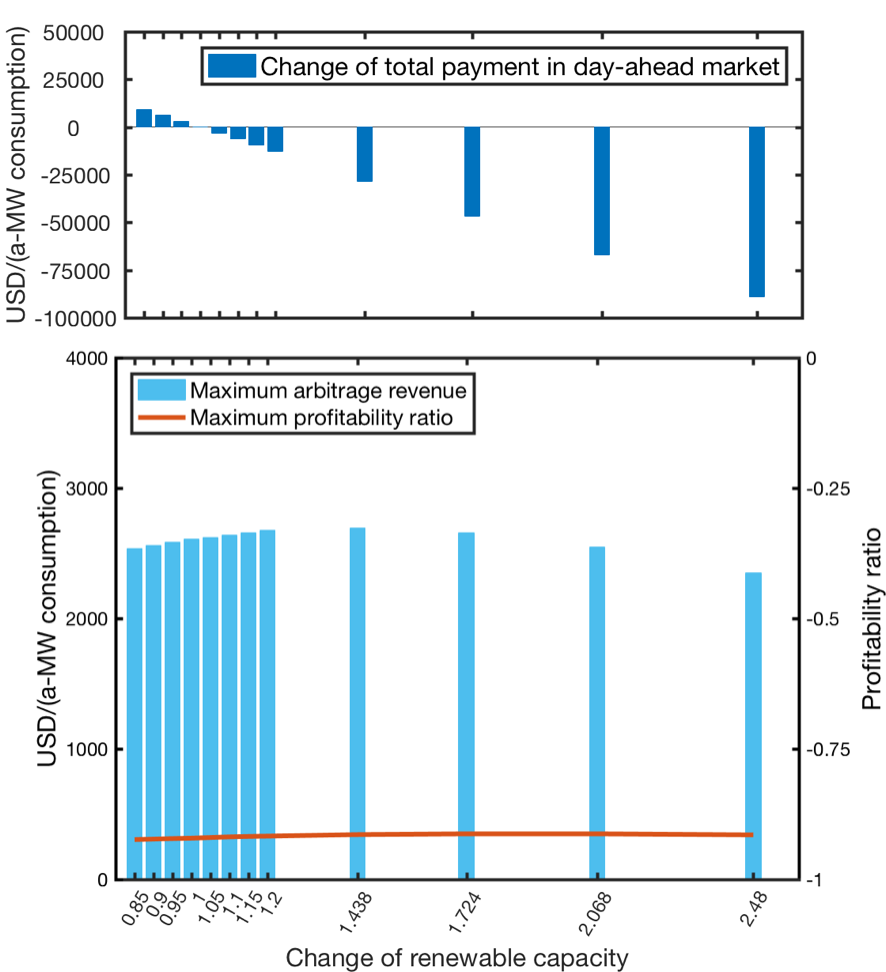
\includegraphics[width=0.95\linewidth]{Figures/RenewablePenetration_PJM}
	\caption{Impacts of renewable generations on revenue and profitability of arbitrage using flexibility as well as on total amount of transations in day-ahead market in PJM}
	\label{fig:renew_pjm}
\end{figure}

PJM reported that it had received negative offers from wind generation enabled by the federal wind production tax credit (PTC)\cite{PJM_price_limit_1}. However, without a clear framework of negative price formation, predictive studies would hardly be robust. 

\subsection{Sensitivity analysis}
\label{sec:sensitivity}
Throughout the whole study, there are two crucial assumption made, i.e. the perfect predictability assumption and fixed price assumption. Elaborated in the literature, this two assumptions are common pragmatic ways in similar studies to indicate a idealistic value as upper bound. Nonetheless, it is necessary to study how reliable the results are based on these assumptions. Besides, the sensitivities of other parameters that were determined based on assumptions are also tested in this section.

\subsubsection{Limited predictability}
Validity and issues regarding this assumption was elaborated in Section \ref{sec:perfect-forecast} in the literature review. In reality, players have a set of methods to forecast the price in short run, some of which are quite efficient and accurate \cite{Weron2014} so close to the perfect forecast assumption. However, while valuing the total market, we shall view the market as whole where players' ability of predicting vary significantly. Therefore, here we would calculate the maximum deviations from our previous estimations in a worst case scenario, i.e. derive lower bounds, where players' forecasting ability is poor. This worst forecast method is defined as ``backcast" as is explained in Section \ref{sec:perfect-forecast}, via which market participates directly take the historical price to foresee the future price. This is the simplest way of forecasting the price and is feasible for all players without the needs for any modeling abilities, so shall indeed represent the lowest possible values.

We tested two scenarios where the price is lagged by 1 day and 1 week respectively, i.e. taking the day-ahead and week-ahead price as the predicted price. The results are summarized in Table \ref{tab:sensitivity-predict-germany} to \ref{tab:sensitivity-predict-nsw}.

 \begin{table}[h!]
 	\centering
 	\begin{tabular}{L{3.6cm} R{2cm} R{2cm} R{2cm} R{2cm}}
 		\hline
 		 \textbf{Case} & \multicolumn{2}{c}{\textbf{Backcast - 1 week}} & \multicolumn{2}{c}{\textbf{Backcast - 1 day}} \\
 		 & MR\footnote{Max. Revenue: difference in percentage }& MPR\footnote{Max. Profitability Ratio: difference in percentage point}& MR$^a$ & MPR$^b$ \\
 		 \hline
 		 \multicolumn{5}{l}{\textbf{ESS} }\\
 		 DA & -50.6\%& -2.3\% & -48.9\%& -2.1\% \\
 		 ID & -50.0\%& - 3.2\%&-52.5\%  & -4.1\%\\
 		 BE & -133.1\%& - 131.8\%&-101.3\%  & -112.2\%\\
 		 PCR & -0.0\%& - 0.0\%&N.A.\footnote{Primary and secondary control markets are organized by weekly auctions} & N.A.$^c$\\
 		 SCR & -10.3\%& - 0.6\%& N.A.$^c$ & N.A.$^c$ \\
 		 DA+ID & -52.3\%& - 4.1\%& -52.1\% & -4.7\% \\
 		 DA+ID+SCR & -35.9\%& - 0.9\%& -38.6\% & -1.3\% \\
 		 DA+ID+PCR+SCR & -33.3\%& - 0.0\%& -33.0\% & -0.1\% \\
 		 \hline
 		 \multicolumn{5}{l}{\textbf{EV2G} }\\
 		 DA & -36.1\%& -1.2\% & -58.6\% &-1.8\% \\
 		 DA+ID & -41.5\%& -2.3\% & -59.0\% &-3.0\% \\
 		 DA+ID+SCR & -22.3\%& -1.1\% & -30.4\% &-1.6\% \\
 		 DA+ID+PCR+SCR & -11.6\%& -1.1\% & -22.0\% &-1.5\% \\
 		 \hline
 	\end{tabular}
 \caption{Summary of sensitivity analysis on predictability in Germany}\label{tab:sensitivity-predict-germany}
 \end{table}

First of all, it can be noticed the results for providing balancing energy dropped considerably, which verified our previous analysis that this market is not practically feasible for market players due to the volatility and unpredictability of balancing energy price, reBAP. 

Besides, we can see the cases involving arbitrage is more sensitive than cases with frequency control services. This implies that predicting price precisely for selling frequency control reserves is not as a critical issue as for arbitrage.

Finally, it was found while backcast for 1 day had sightly better performance than backcast for 1 week for ESS, the situation reversed for EV2G. This can be explained because EV driving behaviors embedded in our model also have a weekly pattern, as was shown in preceding section. It is necessary to matching EV driving profiles well with the price profiles.

 \begin{table}[h!]
	\centering
	\begin{tabular}{L{3.6cm} R{2cm} R{2cm} R{2cm} R{2cm}}
		\hline
		\textbf{Case} & \multicolumn{2}{c}{\textbf{Backcast - 1 week}} & \multicolumn{2}{c}{\textbf{Backcast - 1 day}} \\
		& MR\footnote{Max. Revenue: difference in percentage }& MPR\footnote{Max. Profitability Ratio: difference in percentage point}& MR$^a$ & MPR$^b$ \\
		\hline
		\multicolumn{5}{l}{\textbf{ESS} }\\
		DA & -35.5\%& -1.9\% & -17.9\%& -1.1\% \\
		RegD & -4.4\%& -6.4\%&-4.4\%  & -5.1\%\\
		RegA & -33.3\%& -22.4\%&-26.7\%  & -19.3\%\\
		DA+RT & -51.6\%& - 7.2\%&  -39.5\%& -6.1\% \\
		DA+RT+RegD & -47.8\%& -5.4\%& - 36.7\%& -4.5\%\\
		DA+RT+RegA & -48.6\%& - 12.9\%& -37.2\% & -11.2\% \\
		DA+RT+RegD+RegA & -48.4\%& - 10.3\%& -34.7\% & -8.7\% \\
		\hline
		\multicolumn{5}{l}{\textbf{EV2G} }\\
		DA & -32.9\%& -0.9\% & -18.3\% &-0.6\% \\
		DA+RT & -50.3\%& -3.2\% & -43.8\% &-1.0\% \\
		DA+RT+RegD & -39.5\%& -2.5\% & -34.8\% &-2.3\% \\
		DA+RT+RegA & -41.9\%& -4.1\% & -36.4\% &-3.5\% \\
		DA+RT+RegD+RegA& -34.4\%& -4.1\% & -29.9\% &-3.5\% \\
		\hline
	\end{tabular}
	\caption{Summary of sensitivity analysis on predictability in PJM}\label{tab:sensitivity-predict-pjm}
\end{table}

Compared to results in Germany, the sensitivity of predictability shows a similar pattern. The revenue reduction is less significant in PJM's day-ahead market compared to Germany, implying a more stable price profile.  This can be explained that a power pool with capacity obligation can maximize the participation of all resources and suppress virtual transactions, thereby leading to a robuster price formation than a power exchange. Revenue potential from RegD altered sightly while the value from RegA significantly dropped. This is because in the original plans players were assigned with perfect predictability of frequency control signal as well so that they were able to better tackle the non-energy-neutral signal.  In reality, frequency control signals are impossible to forecast. Therefore, the merit of energy-neutral signal is again demonstrated. However, it shall be emphasized again that implementing energy-neutral signals is a complex and challenging task. A energy-neutral signal might be most beneficial to the system, since it might move to the same direction as the error in order to maintain energy neutrality. This is the rationale why PJM re-engineered the RegD to be conditional energy neutral. 

\begin{table}[h!]
	\centering
	\begin{tabular}{L{2.5cm} R{2cm} R{2cm} R{2cm} R{2cm}}
		\hline
		\textbf{Case} & \multicolumn{2}{c}{\textbf{Backcast - 1 week}} & \multicolumn{2}{c}{\textbf{Backcast - 1 day}} \\
		& MR\footnote{Max. Revenue: difference in percentage }& MPR\footnote{Max. Profitability Ratio: difference in percentage point}& MR$^a$ & MPR$^b$ \\
		\hline
		\multicolumn{5}{l}{\textbf{ESS} }\\
		RT & -58.8\%& -16.6\% & -47.6\%& -14.7\% \\
		\hline
		\multicolumn{5}{l}{\textbf{EV2G} }\\
		RT & -56.4\%& -13.8\% & -51.3\% &-12.7\% \\
		\hline
	\end{tabular}
	\caption{Summary of sensitivity analysis on predictability in NSW}\label{tab:sensitivity-predict-nsw}
\end{table}

In NSW, although we have pointed out the higher volatility in its real-time markets leads to a higher potential of arbitrage compared to markets in Germany and PJM, it also demands higher precision of price forecasting. The revenue and profitability dropped more sensitively than arbitrage cases in the other two geographies.

\subsubsection{Responsive price}
While the amount of flexibility reaches a significant level, their trading behaviors will certainly disturb the market and affect the price. Especially in the case of arbitrage where the price volatility is being utilized for value creation, the actual revenue would be more sensitively depending on the responsive price effect. Regarding frequency control market, the revenue relies on the average price level rather than the price volatility and the distinct price formation mechanism such as the pay-as-bid mode in German markets shall suppress significant disturbances of new players on market price. 

Therefore, we studied the effect only on wholesale energy markets here. It shall be firstly pointed out, with a responsive price, there are still two distinct scenarios exist, i.e. price taker and price marker. In the price taker scenario, although the players' actions will affect the price formation, the market is highly competitive so each player has negligible market power. In contrast, price maker may exist in some markets where the competitions are sufficient and few players can strategically exert its market power to distort the market price. Among these two cases, it is clear that the price taker scenario would indicate a lower bound while price makers are more likely to receive higher payments or better fulfill their strategic goals. Therefore, in this section, we take the worst case scenario where players have no market power. It shall be noticed that in this scenario, their price forecast is not imperfect since the price formation takes place after their decisions are made. 

The results for the day-ahead market in Germany as an illustrating example is shown by Table

\textit{(To be continued)}
\subsubsection{Sensitivity analysis of other parameters}





